\documentclass{jsarticle}

\usepackage[top=30mm, bottom=36mm, left=28mm, right=28mm]{geometry}
\usepackage[yyyymmdd]{datetime}
\usepackage[dvipdfmx]{graphicx}
\usepackage[subrefformat=parens]{subcaption}
\usepackage{listings}
\usepackage{amsmath,amssymb}

\usepackage{../common/mytitle}

\title{データ解析特論 第2回}
\author{201720690 小松 弘人}
\date{\today}

\makeatletter
\def\mojiparline#1{
    \newcounter{mpl}
    \setcounter{mpl}{#1}
    \@tempdima=\linewidth
    \advance\@tempdima by-\value{mpl}zw
    \addtocounter{mpl}{-1}
    \divide\@tempdima by \value{mpl}
    \advance\kanjiskip by\@tempdima
    \advance\parindent by\@tempdima
}
\makeatother
\def\linesparpage#1{
    \baselineskip=\textheight
    \divide\baselineskip by #1
}

\begin{document}
\maketitle
\subsection*{2 正規分布}
\subsubsection*{(1)}
一様乱数をたくさん足し合わせた数の分布は正規分布に近づいていくか,
確認しよう.

\subsubsection*{スクリプト}
\begin{lstlisting}[basicstyle=\ttfamily\footnotesize, frame=single]
# 初期化
N <- 0; data <- 0
f <- function(data, N) {
  # 描画デバイスの作成
  pdf(sprintf("02\\hist%02d.pdf", N), width=10, height=10)
  hist_dev = dev.cur()
  pdf(sprintf("02\\qq%02d.pdf", N), width=10, height=10)
  qq_dev = dev.cur()

  # データの加算とグラフ表示
  data <- data + runif(10000)
  dev.set(hist_dev)
  hist(data)
  dev.set(qq_dev)
  qqplot(qnorm(ppoints(10000)), data)

  dev.off(hist_dev)
  dev.off(qq_dev)
  return(data)
}

# p-valueが大きければ正規分布であると判断できる
N <- N + 1; data <- f(data, N); ks.test(data, "pnorm", mean(data), sd(data))

# 後処理
rm(N, f, data)
\end{lstlisting}

\subsubsection*{結果}
一様乱数を足し合わせたデータのヒストグラムを図\ref{img:hist},
分布を正規分布と比較した際のQ-Qプロットを図\ref{img:qqplot}に示す.
また,Kolmogorov-Smirnov検定を行った際のp値の値を\ref{tbl:ks.test}に示す.

\subsubsection*{考察}
図\ref{img:hist}のヒストグラムから,加算した回数が増えるごとに
分布が正規分布に近づいていることが分かる.
また,図\ref{img:qqplot}のQ-Qプロットから,加算した回数が増えるごとに
プロットが直線に近づいていることが分かる.
Q-Qプロットは,比較した2つの分布が似ているほどプロットが直線に近づく.
したがって,正規分布に近づいていることが確認できる.
さらに,表\ref{tbl:ks.test}から,加算した回数が増えるごとに
p値が増加していることが分かる.
Kolmogorov-Smirnov検定では,p値が高ければ,そのデータの分布は
正規分布に基づいているといえる.
したがって,表\ref{tbl:ks.test}からも正規分布に近づいていくことが分かる.

\begin{figure}[b]
	\centering
	\begin{minipage}{0.8\hsize}
		\centering
		\begin{tabular}{c}
			\begin{minipage}{0.25\hsize}
				\centering
				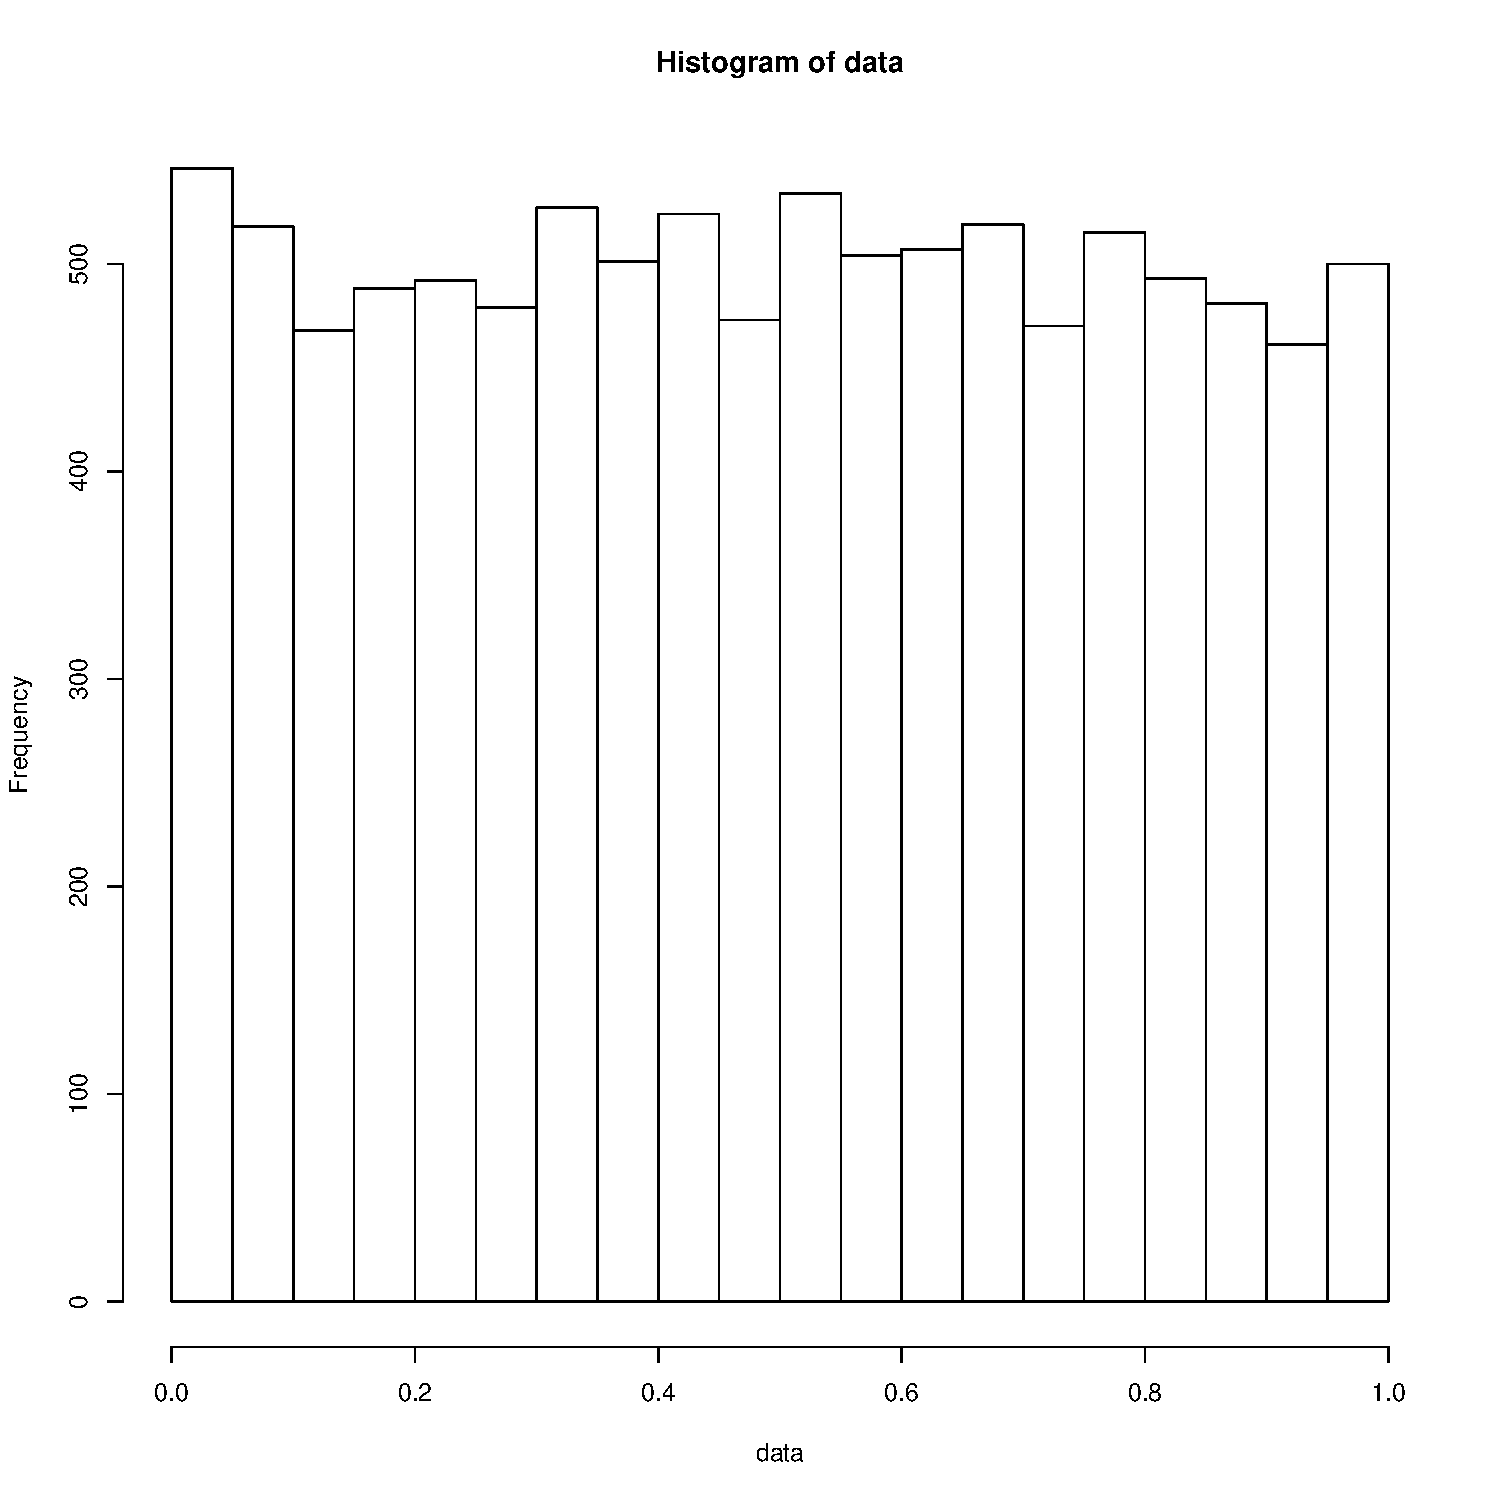
\includegraphics[width=\linewidth]{img/hist01.pdf}
				\subcaption{初期化 (一様乱数)}
			\end{minipage}
			\begin{minipage}{0.25\hsize}
				\centering
				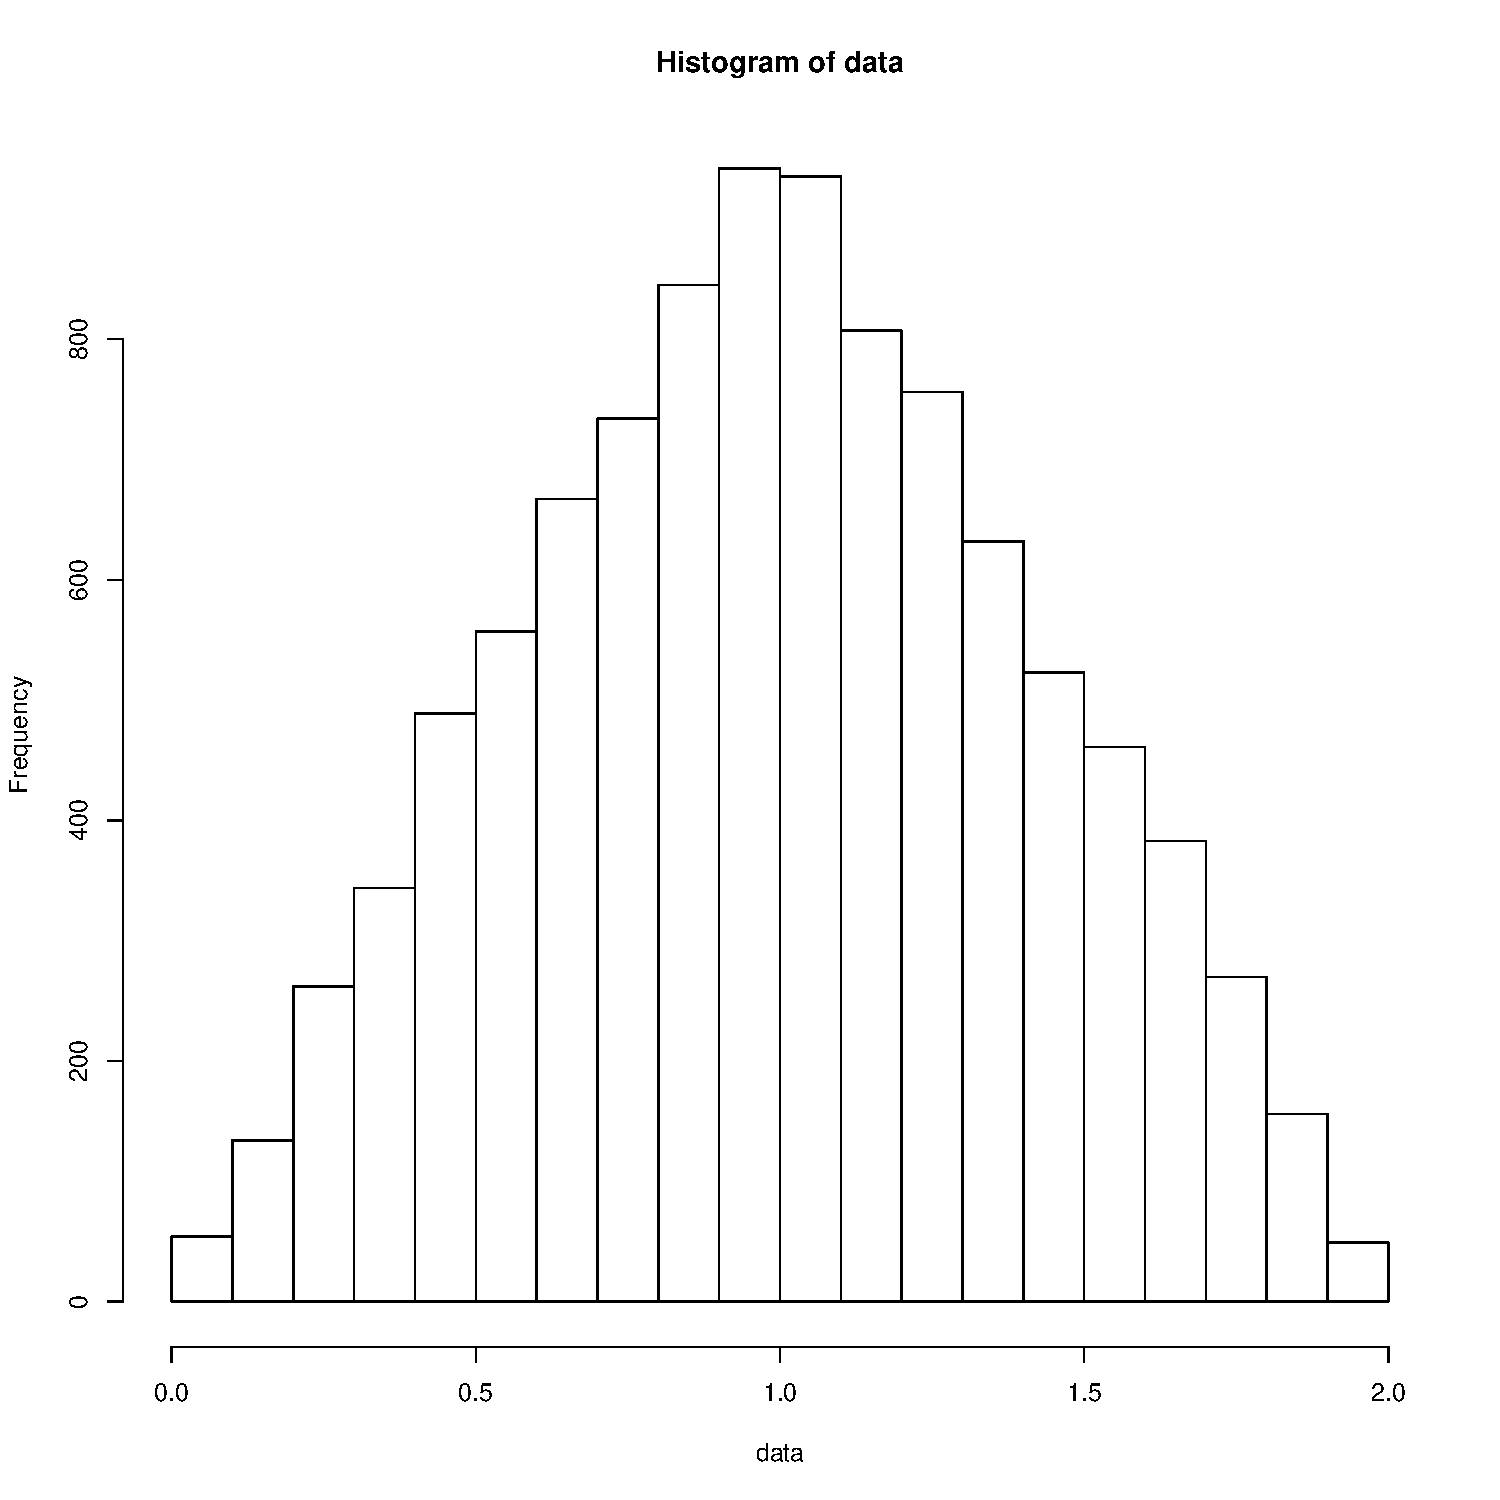
\includegraphics[width=\linewidth]{img/hist02.pdf}
				\subcaption{1回目}
			\end{minipage}
			\begin{minipage}{0.25\hsize}
				\centering
				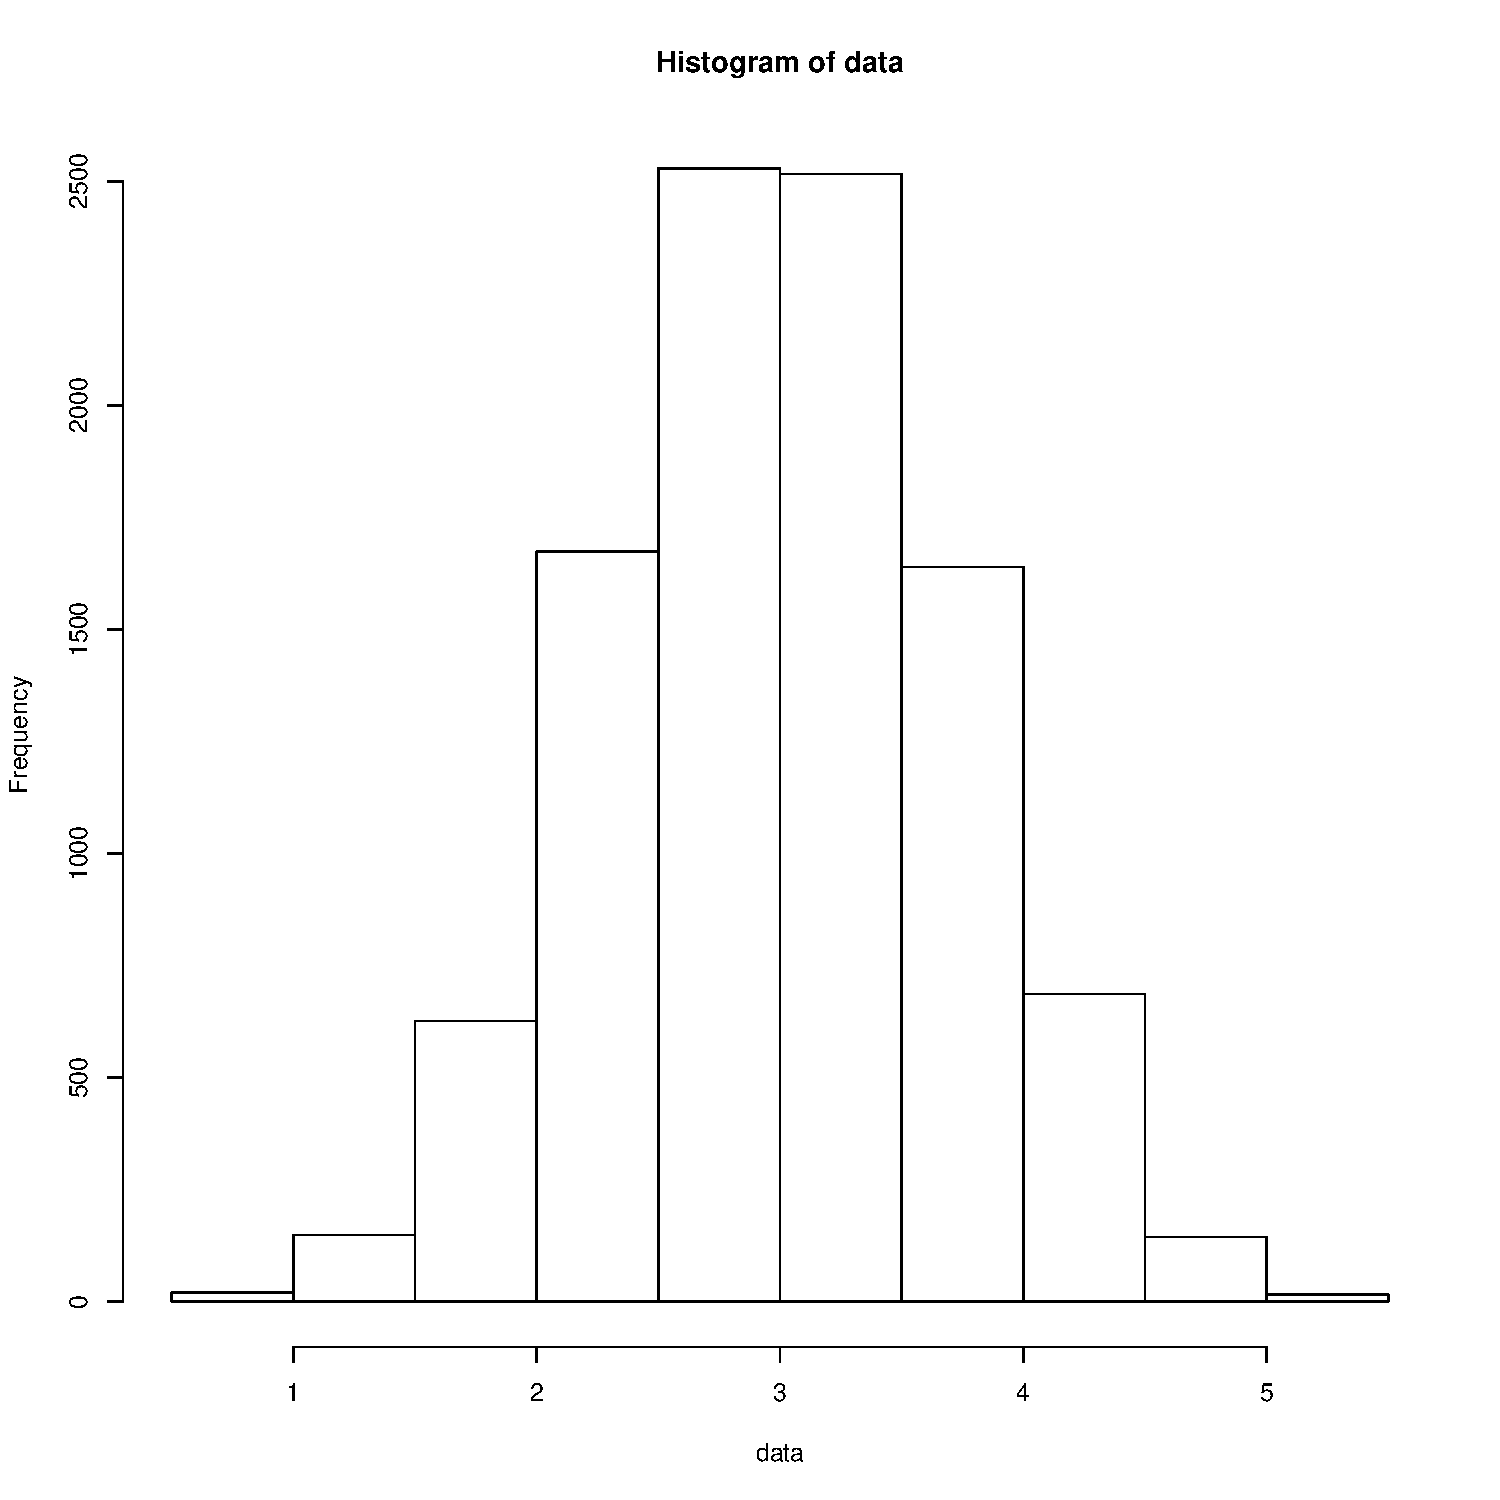
\includegraphics[width=\linewidth]{img/hist06.pdf}
				\subcaption{5回目}
			\end{minipage}
			\begin{minipage}{0.25\hsize}
				\centering
				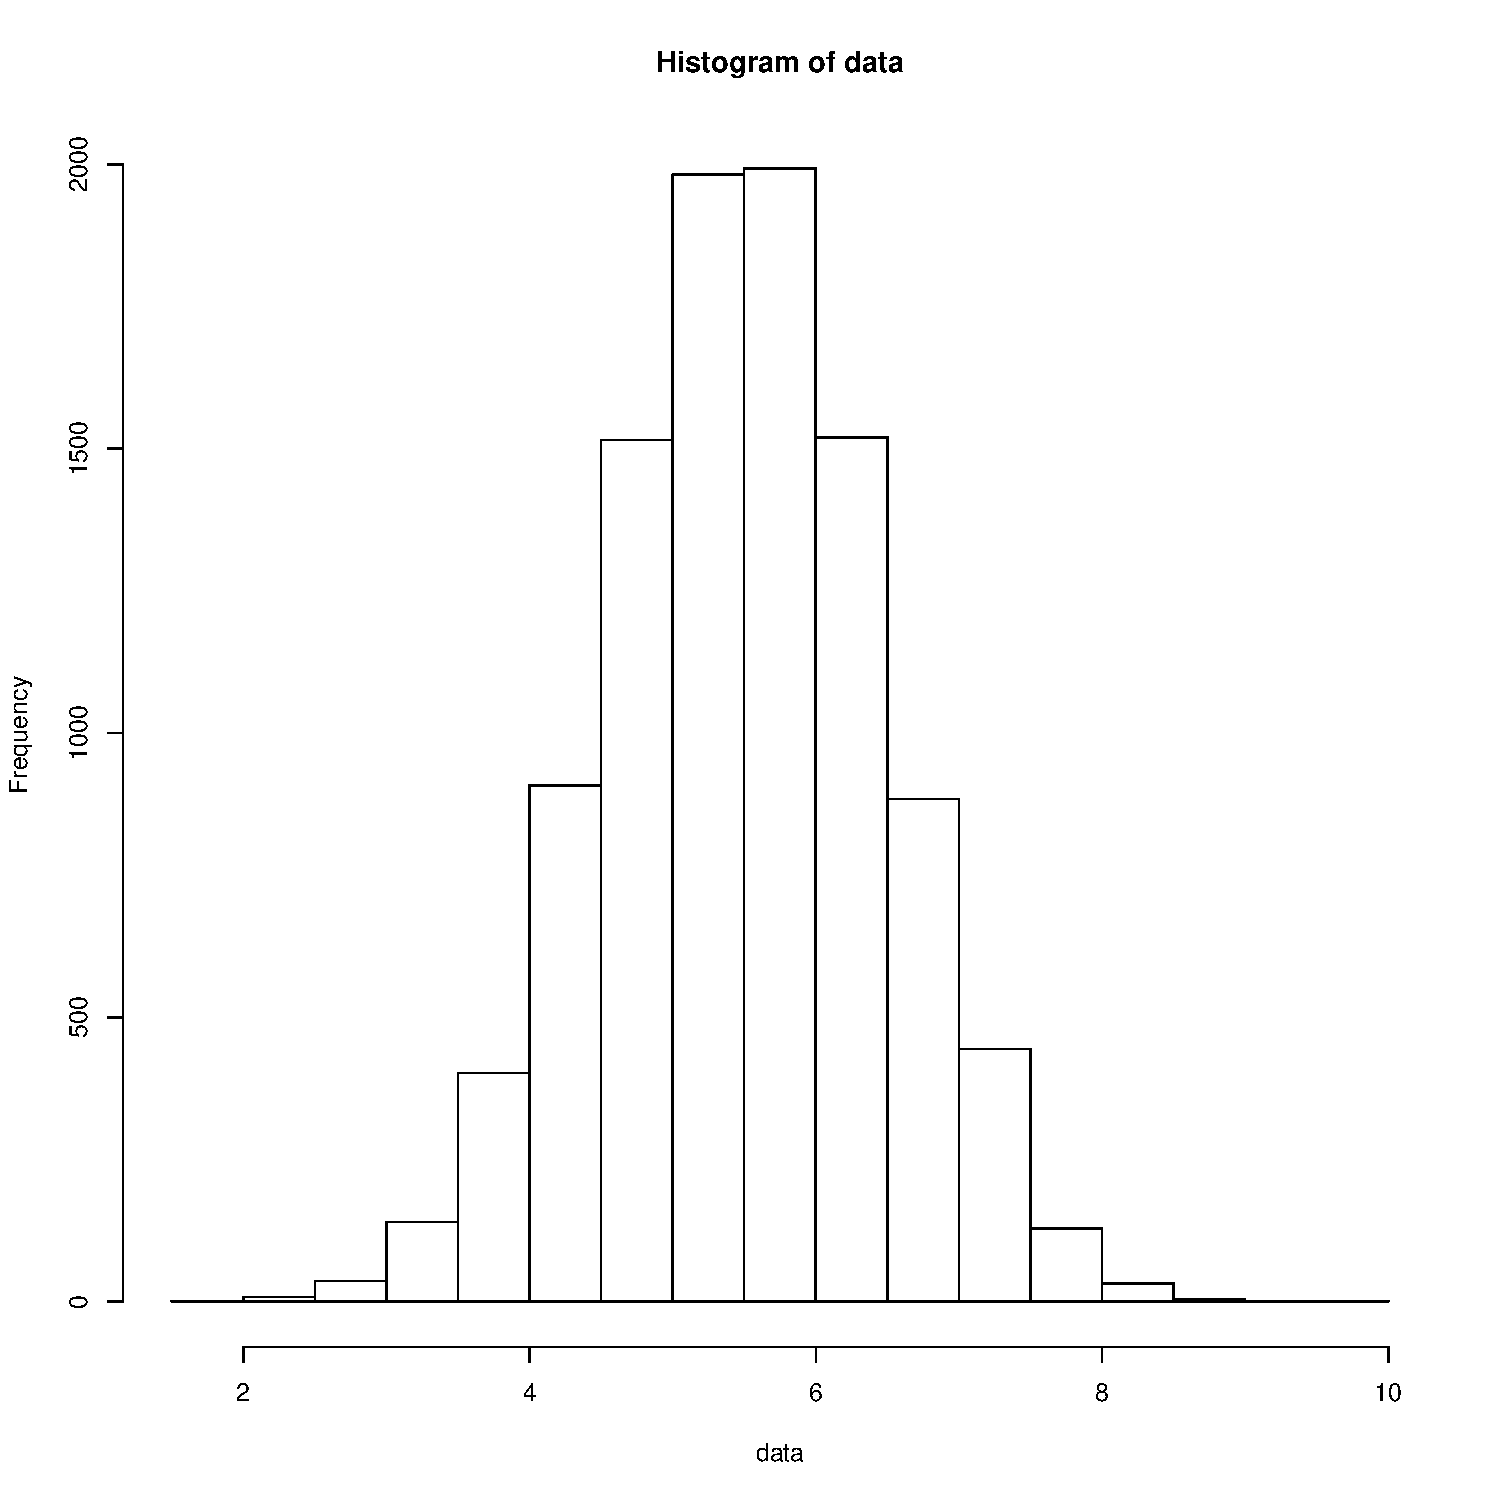
\includegraphics[width=\linewidth]{img/hist11.pdf}
				\subcaption{10回目}
			\end{minipage}
		\end{tabular}
		\caption{ヒストグラム}
		\label{img:hist}
	\end{minipage}
	\begin{minipage}{0.8\hsize}
		\centering
		\begin{tabular}{c}
			\begin{minipage}{0.25\hsize}
				\centering
				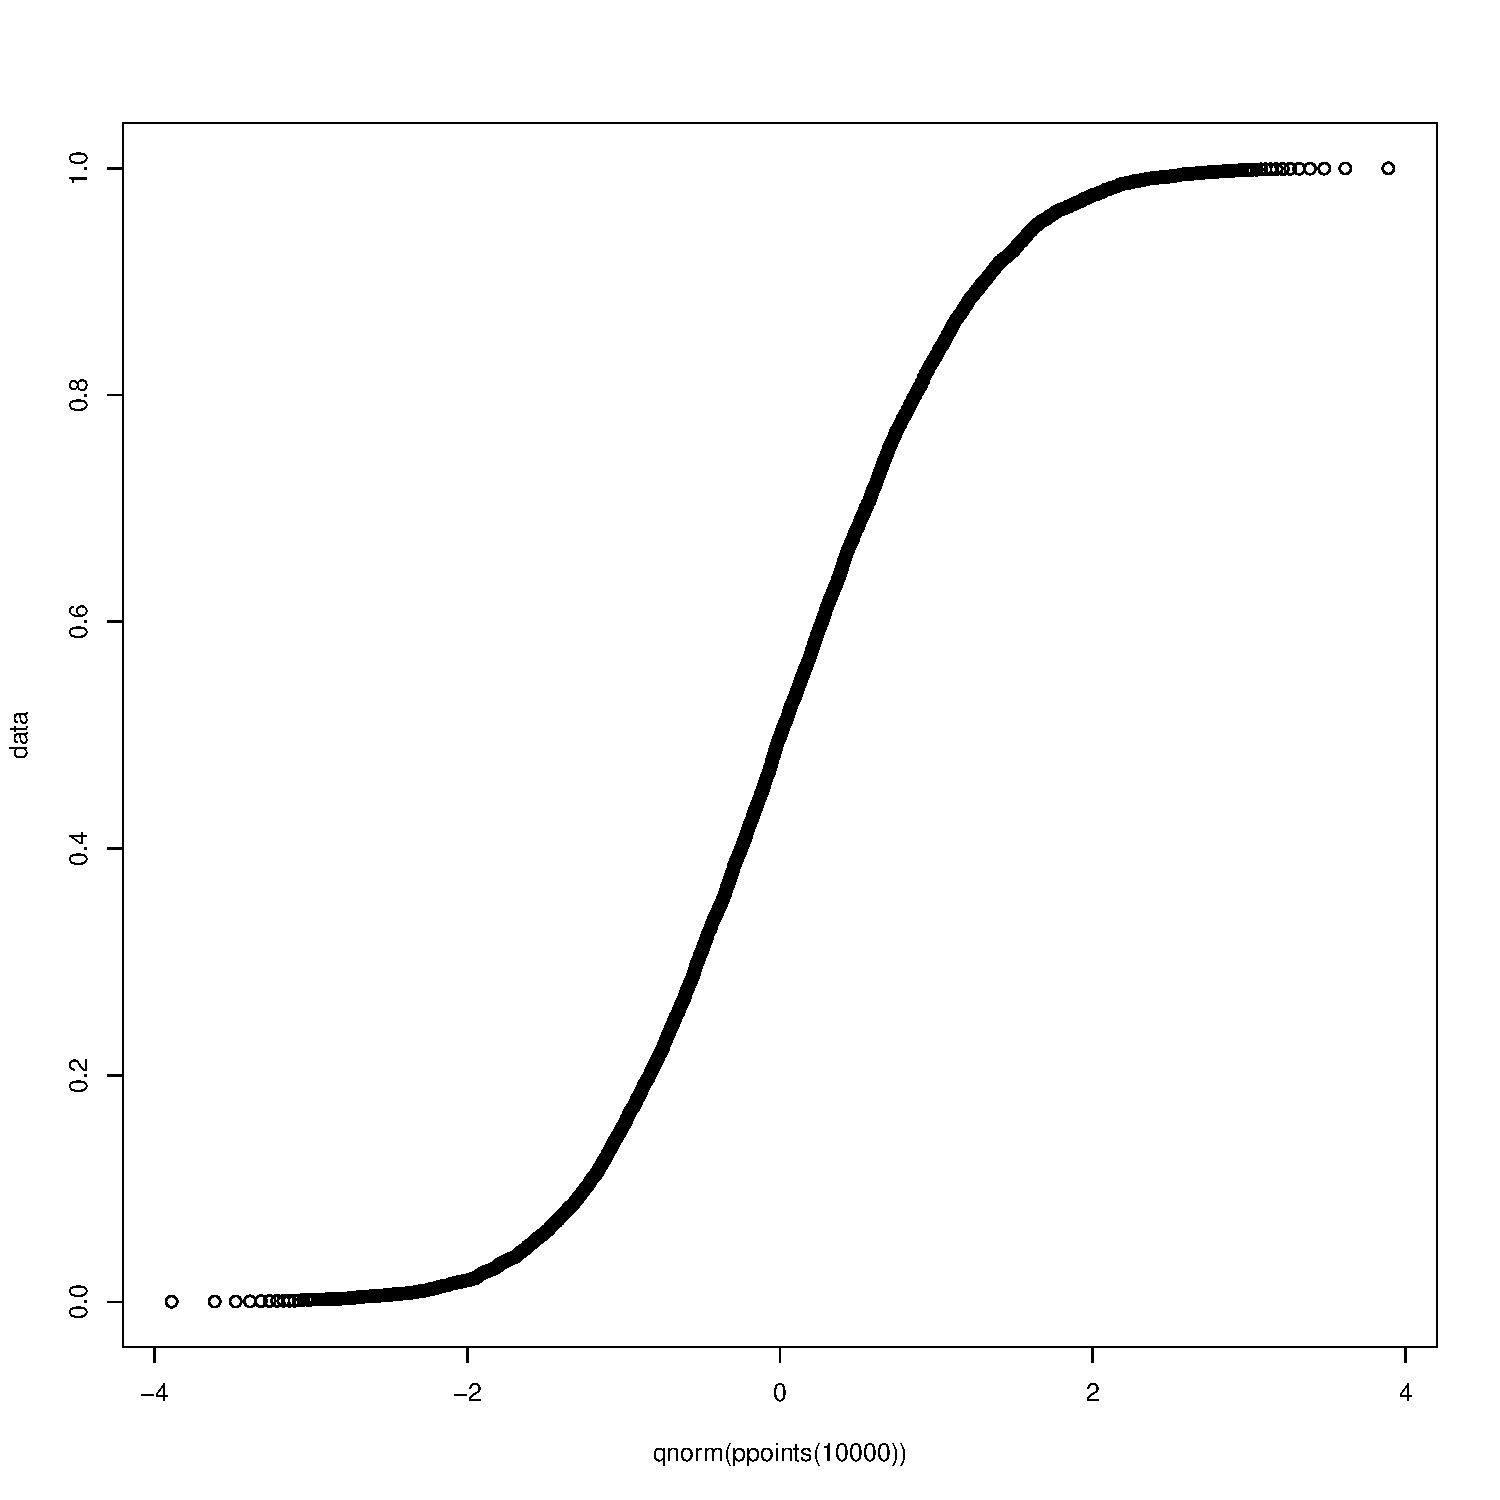
\includegraphics[width=\linewidth]{img/qq01.pdf}
				\subcaption{初期化 (一様乱数)}
			\end{minipage}
			\begin{minipage}{0.25\hsize}
				\centering
				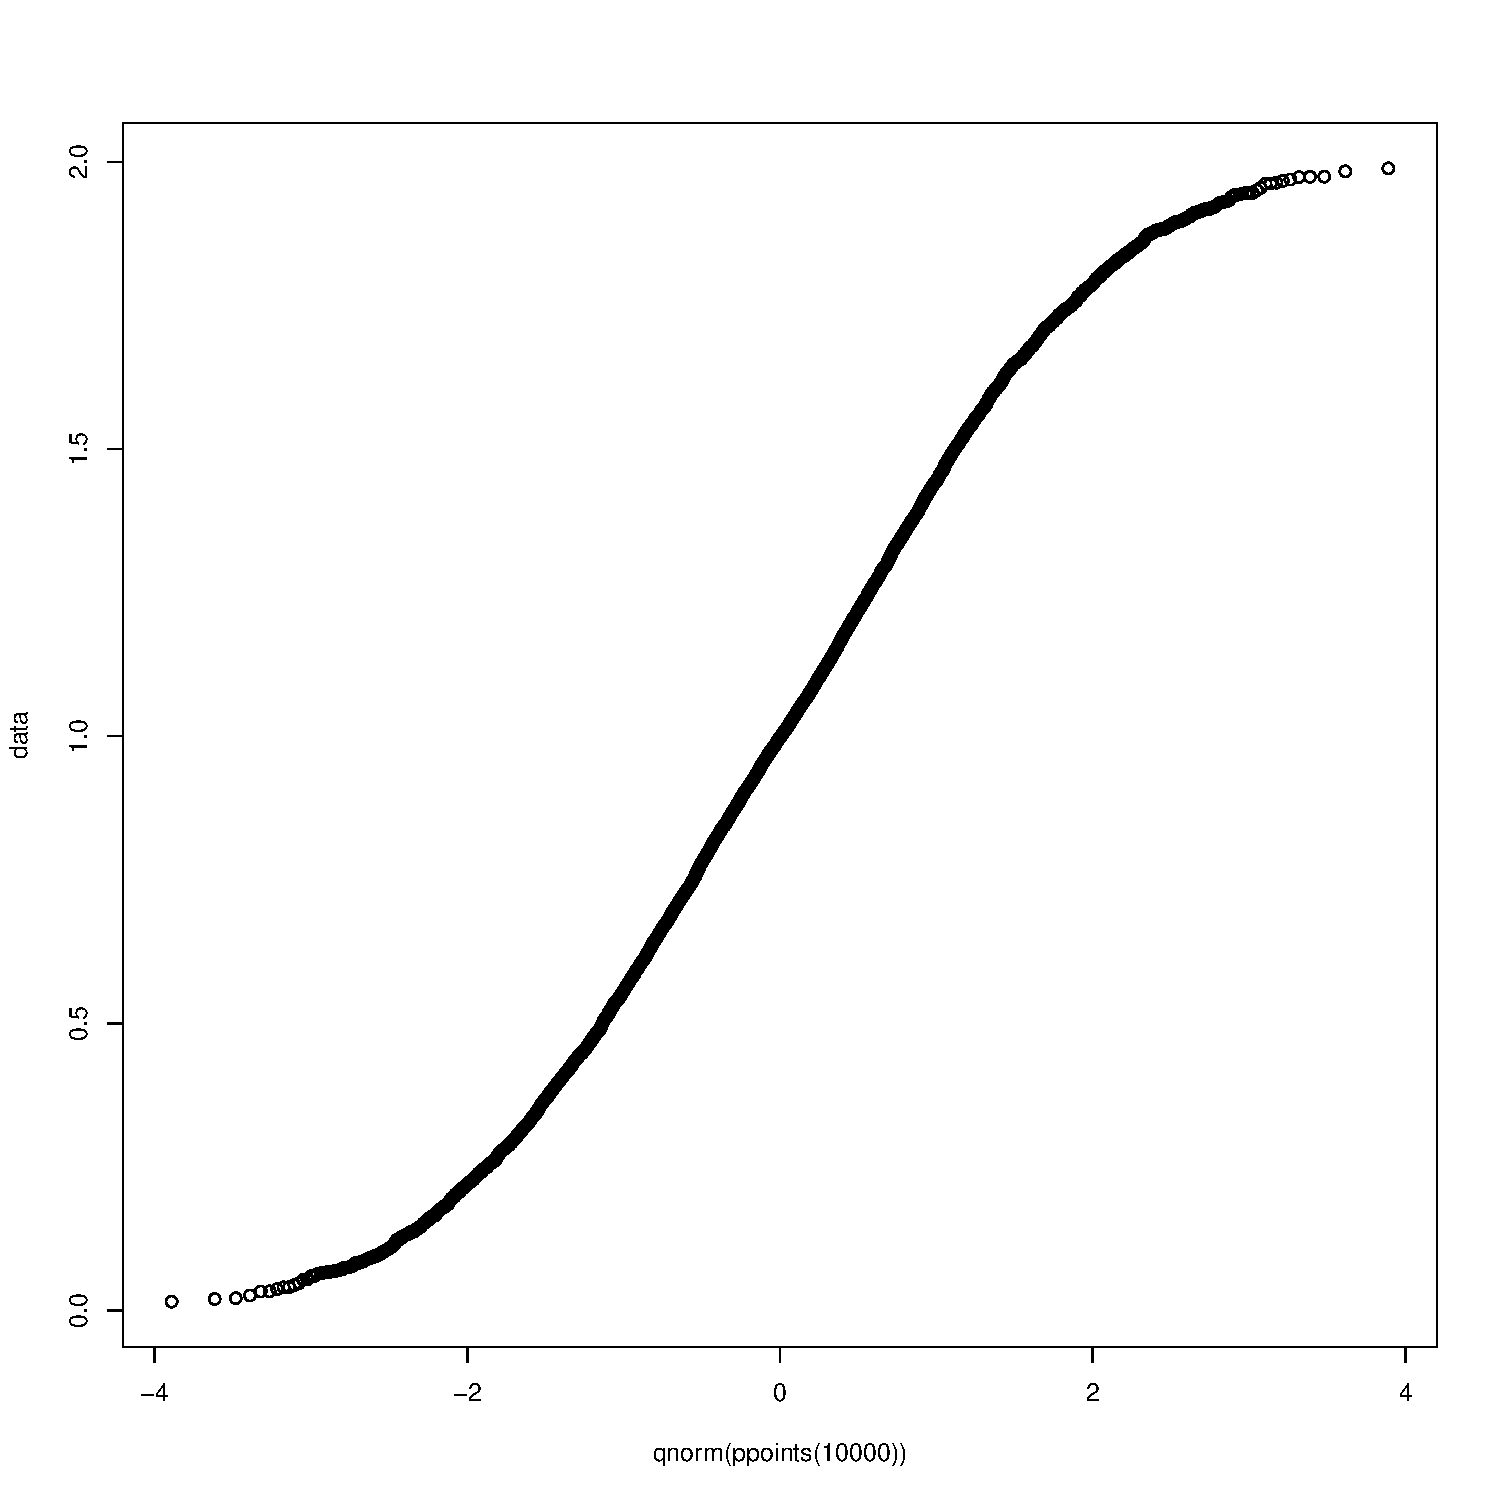
\includegraphics[width=\linewidth]{img/qq02.pdf}
				\subcaption{1回目}
			\end{minipage}
			\begin{minipage}{0.25\hsize}
				\centering
				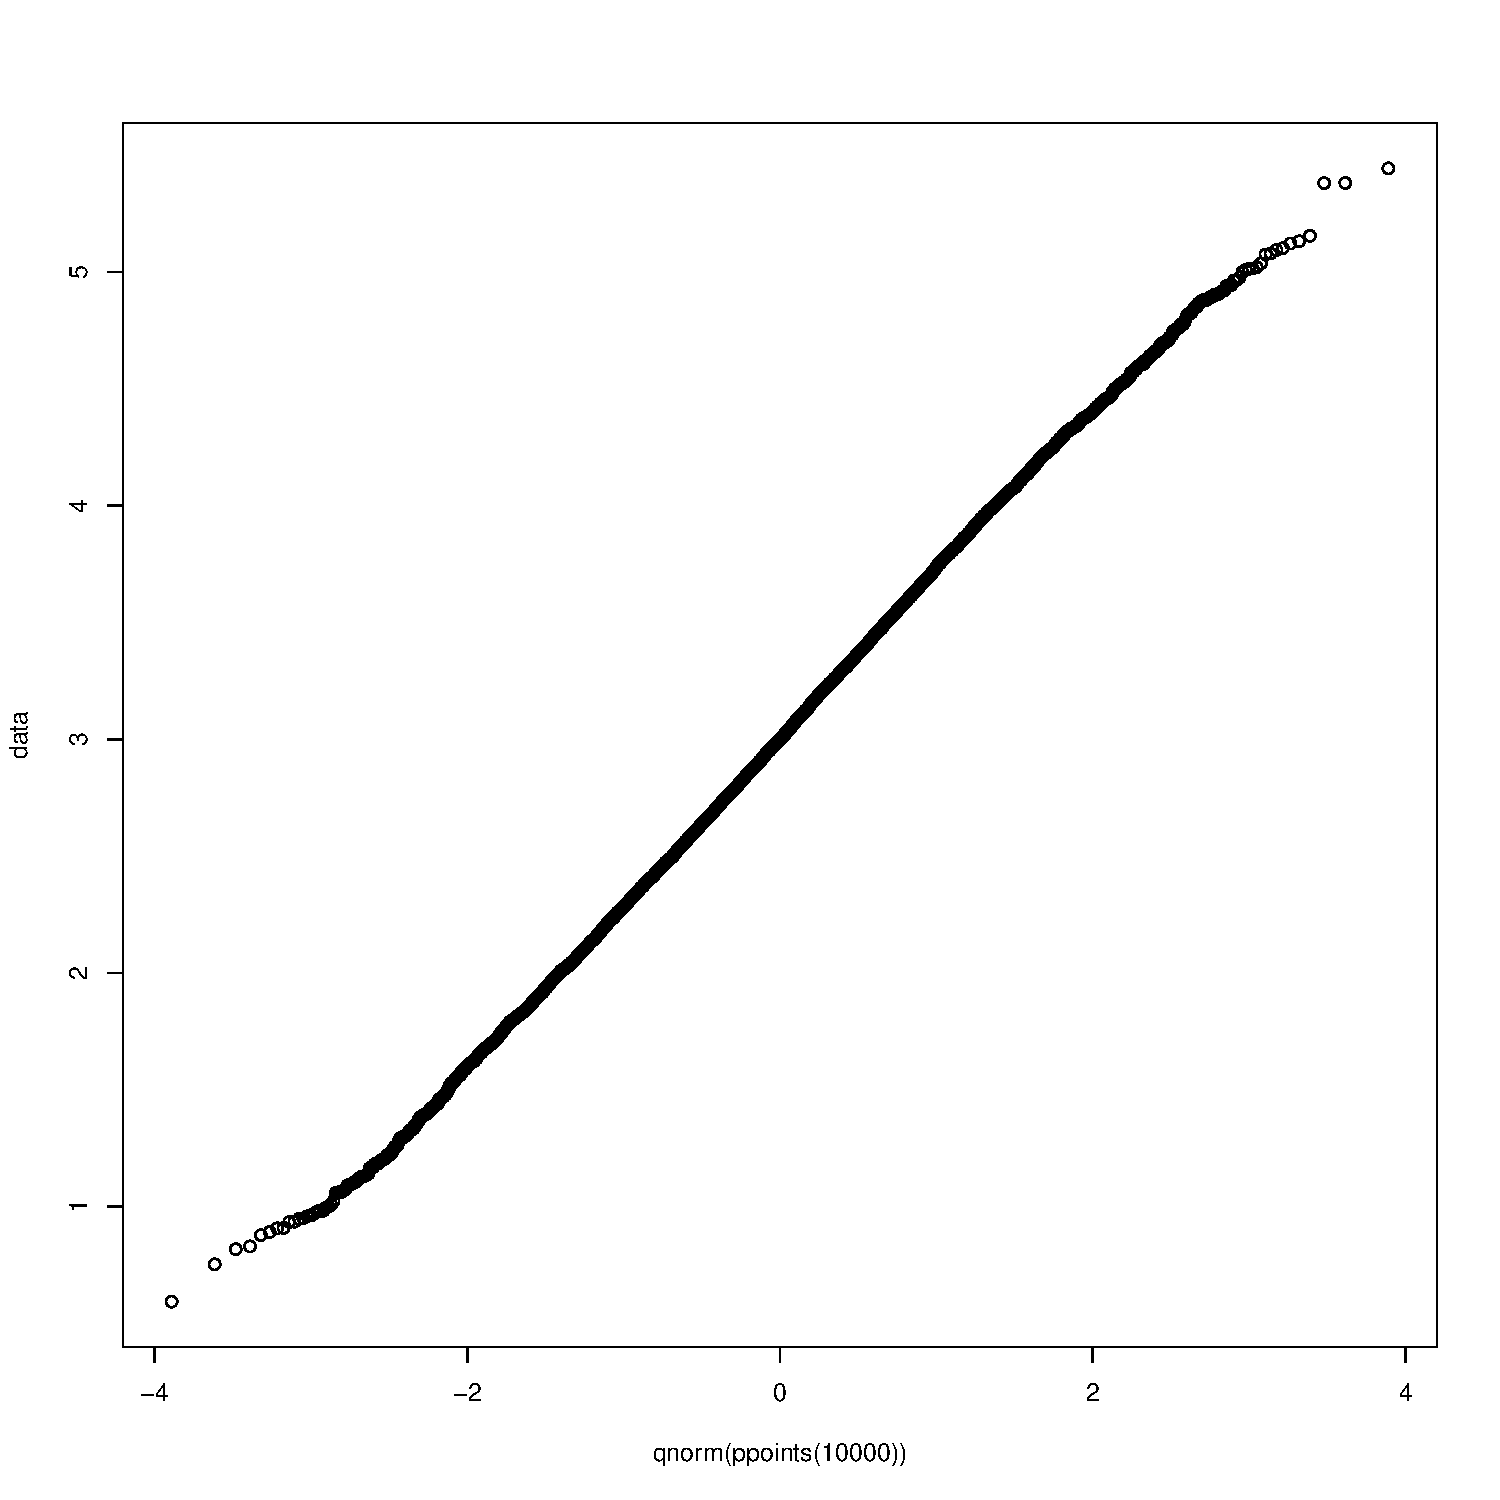
\includegraphics[width=\linewidth]{img/qq06.pdf}
				\subcaption{5回目}
			\end{minipage}
			\begin{minipage}{0.25\hsize}
				\centering
				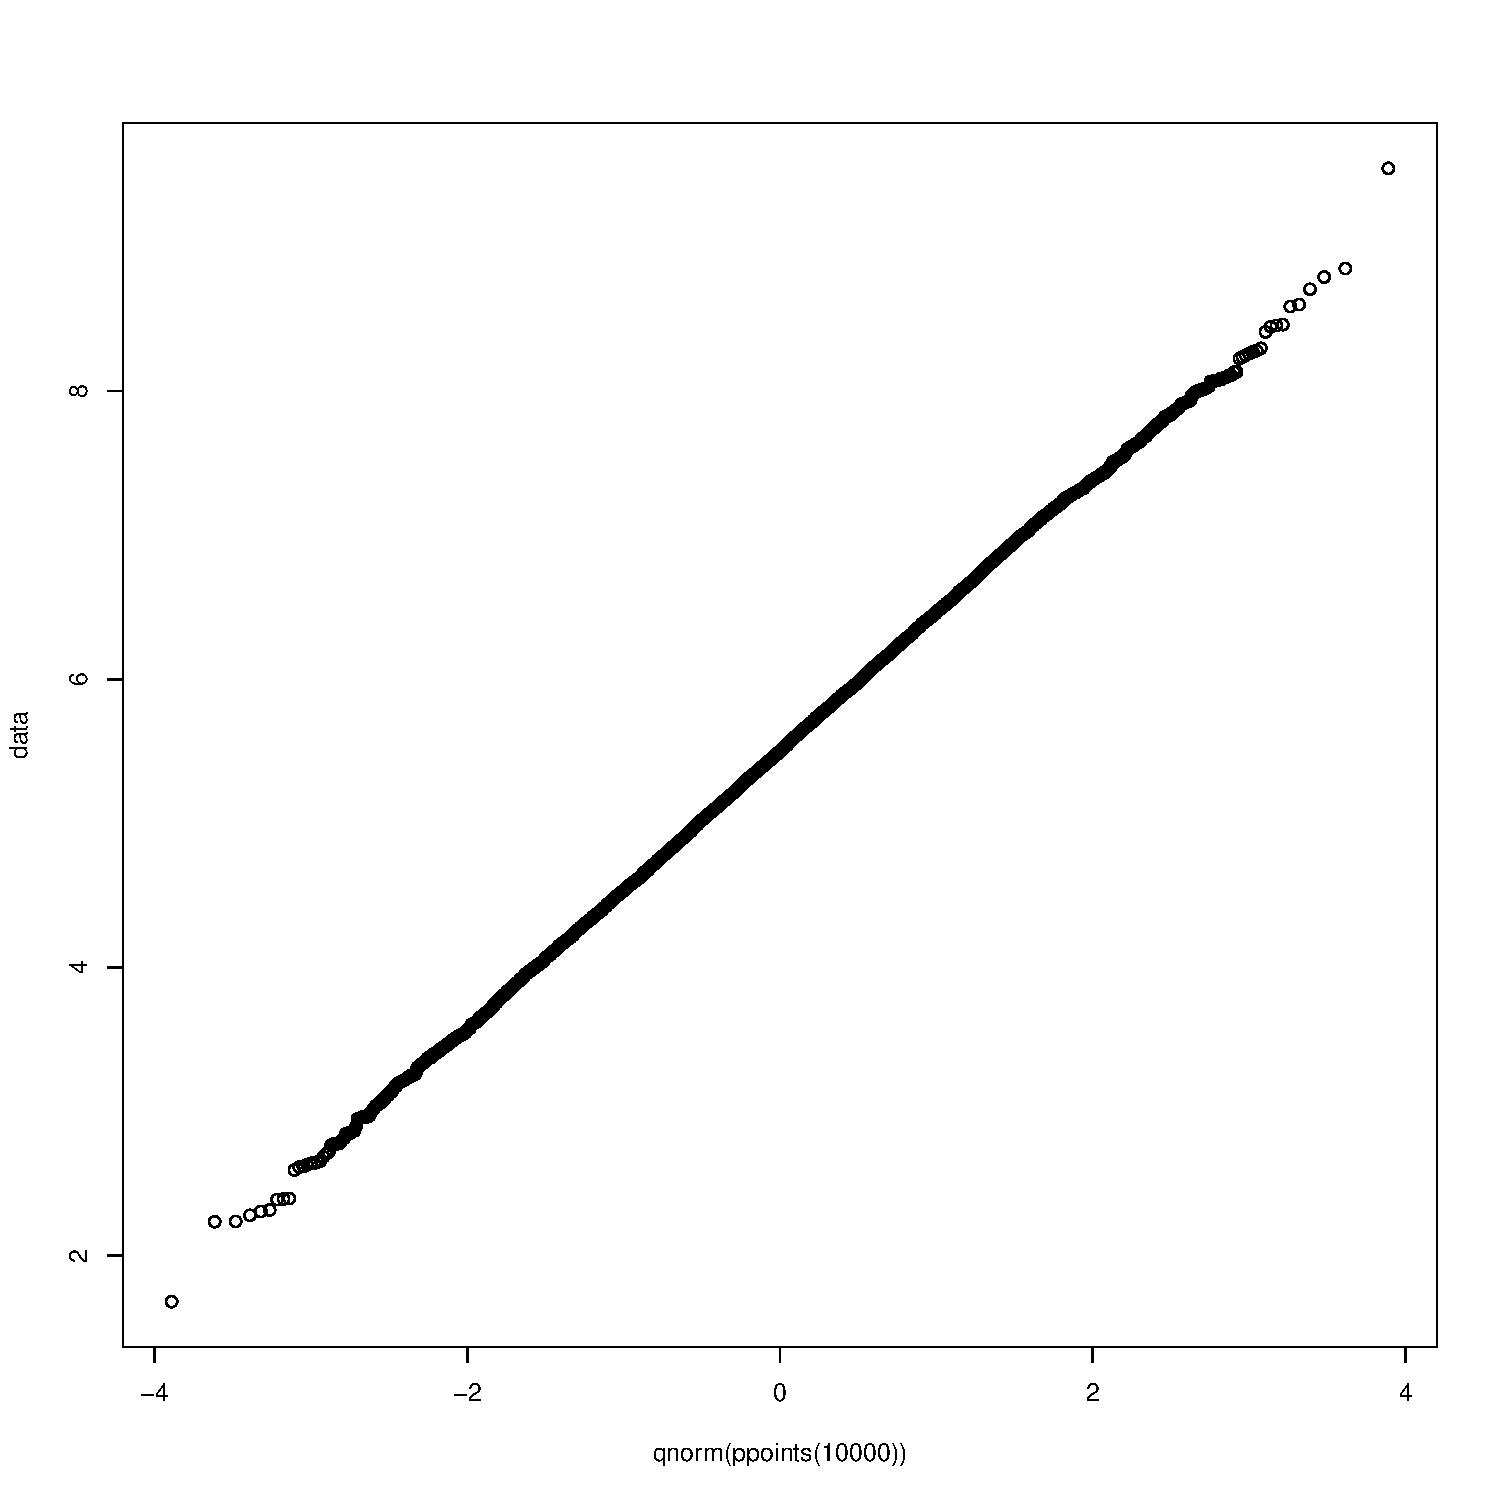
\includegraphics[width=\linewidth]{img/qq11.pdf}
				\subcaption{10回目}
			\end{minipage}
		\end{tabular}
		\caption{Q-Qプロット}
		\label{img:qqplot}
	\end{minipage}
\end{figure}

\begin{table}[b]
	\centering
	\caption{Kolmogorov-Smirnov検定のp値}
	\label{tbl:ks.test}
	\begin{tabular}{c|c|c|c} \hline
		初期化 (一様乱数) & 1回目 & 5回目 & 10回目 \\ \hline
		$2.20\!\times\!10^{-16}$ & 0.000691 & 0.6155 & 0.9611 \\ \hline
	\end{tabular}
\end{table}

\subsection*{4 最尤推定}
\subsubsection*{(1)}
平均,分散の異なる2種の正規乱数を発生させ,その和の分布が
式\ref{eqn:sum-density}で示す結果に一致しているか,
パラメータを最尤推定し確認しよう.

\subsubsection*{和の密度関数}
確率変数$x,y$がそれぞれ密度関数$p_1(x)=\mathcal{N}(x;\mu_1, \sigma_1^2),
p_2(y)=\mathcal{N}(y;\mu_2,\sigma_2^2)$に従うとき,
2つの和$z=x+y$は畳み込み積分に従う.

\begin{equation}
	p(z) = p_1(x) \ast p_2(y) = \int_{-\infty}^{\infty} p_1(z-t)p_2(t) dt
	= \mathcal{N}(z; \mu_1+\mu_2, \sigma_1^2+\sigma_2^2)
	\label{eqn:sum-density}
\end{equation}

\subsubsection*{スクリプト}
\begin{lstlisting}[basicstyle=\ttfamily\footnotesize, frame=single]
data1 <- rnorm(1000000, mean=0.4, sd=1)
data2 <- rnorm(1000000, mean=0.6, sd=2)
data <- data1 + data2

# 最尤推定法 (mle) を使用
library(stats4)
nLL <- function(mean) -sum(dnorm(data, mean, 2, log=T))
(fit <- mle(nLL, start=list(mean=0)))

# 最尤推定法 (optim) を使用
library(stats)
nLL <- function(arg) -sum(dnorm(data, mean=arg[1], sd=arg[2], log=T))
(fit <- optim(c(0,1), nLL))$par

# 後処理
rm(data1, data2, data, nLL)
\end{lstlisting}

\subsubsection*{結果}
スクリプトを実行した結果を以下に示す.
\begin{verbatim}
> nLL <- function(mean) -sum(dnorm(data, mean, 2, log=T))
> (fit <- mle(nLL, start=list(mean=0)))
Call:
mle(minuslogl = nLL, start = list(mean = 0))

Coefficients:
     mean 
0.9990161
> nLL <- function(arg) -sum(dnorm(data, mean=arg[1], sd=arg[2], log=T))
> (fit <- optim(c(0,1), nLL))$par
[1] 0.9997631 2.2365586

\end{verbatim}

\subsubsection*{考察}
$p_1(x)=\mathcal{N}(x;0.4, 1^2) , p_2(y)=\mathcal{N}(y;0.6, 2^2)$に従う
確率変数$x,y$の和$z$の密度関数は
$p(z)=\mathcal{N}(z; 1, 5)$となるはずである.
最尤推定を行ったところ,平均はどちらの手法でも$1$に近い値となった.
また,標準偏差も$\sqrt{5} \fallingdotseq 2.236$と近い値となった.
したがって,式\ref{eqn:sum-density}とほぼ一致すると考えられる.

\subsection*{6 混合分布}
\subsubsection*{(1)}
MASSパッケージに含まれる多変量正規乱数生成関数\verb|mvrnorm()|を使って,
3つのガウス成分からなる混合分布から発生させた,2次元の乱数ベクトル系列を
作成しよう.

\subsubsection*{スクリプト}
以下のような2変数3成分ガウス混合分布に従う確率変数$x$を考える.
\begin{equation}
	p(x)=
	0.2\mathcal{N}(x; \mu_a, \Sigma_a) + 
	0.5\mathcal{N}(x; \mu_b, \Sigma_b) + 
	0.3\mathcal{N}(x; \mu_c, \Sigma_c)
\end{equation}
\begin{equation}
	\mu_a = \left[
		\begin{array}{r}
			-5 \\
			-10
		\end{array}
	\right],
	\Sigma_a = \left[
		\begin{array}{rr}
			4 & 3 \\
			3 & 9
		\end{array}
	\right],
	\mu_b = \left[
		\begin{array}{r}
			0 \\
			0
		\end{array}
	\right],
	\Sigma_b = \left[
		\begin{array}{rr}
			4 & 0 \\
			0 & 4
		\end{array}
	\right],
	\mu_c = \left[
		\begin{array}{r}
			7 \\
			5
		\end{array}
	\right],
	\Sigma_c = \left[
		\begin{array}{rr}
			4 & 0 \\
			0 & 9
		\end{array}
	\right]
	\label{eqn:parameters}
\end{equation}

\begin{lstlisting}[basicstyle=\ttfamily\footnotesize, frame=single]
library(MASS)

# 乱数ベクトル系列作成関数
rgmix <- function(n) {
  y <- c();
  for(i in 1:n) {
    u <- runif(1);
    if(u < 0.2) {
      v <- mvrnorm(1, c(-5, -10), matrix(c(4, 3, 3, 9), 2, 2))
    } else if(u < 0.7) {
      v <- mvrnorm(1, c(0, 0), matrix(c(4, 0, 0, 4), 2, 2))
    } else {
      v <- mvrnorm(1, c(7, 5), matrix(c(4, 0, 0, 9), 2, 2))
    }
    y <- c(y, v)
  }
  y <- matrix(y, ncol=2, byrow=T)
  return(y)
}

# 描画デバイスの作成
pdf("02\\mvrnorm-plot.pdf", width=10, height=10)
dev = dev.cur()

# データ生成
dat <- rgmix(5000)
dat <- data.frame(x=dat[,1], y=dat[,2])

# プロット
dev.set(dev)
plot(dat, xlim=c(-20, 20), ylim=c(-20, 20))
dev.off(dev)
\end{lstlisting}

\subsubsection*{結果}
それぞれの正規分布のみで生成した乱数のプロットを
図\ref{img:mvrnorm-plot}
\subref{img:mvrnorm-plot1}--\subref{img:mvrnorm-plot3},
ガウス混合分布で生成した乱数のプロットを
図\ref{img:mvrnorm-plot}\subref{img:mvrnorm-plot-mix}
に示す.

\begin{figure}[b]
	\centering
	\begin{minipage}{0.8\hsize}
		\centering
		\begin{tabular}{c}
			\begin{minipage}{0.25\hsize}
				\centering
				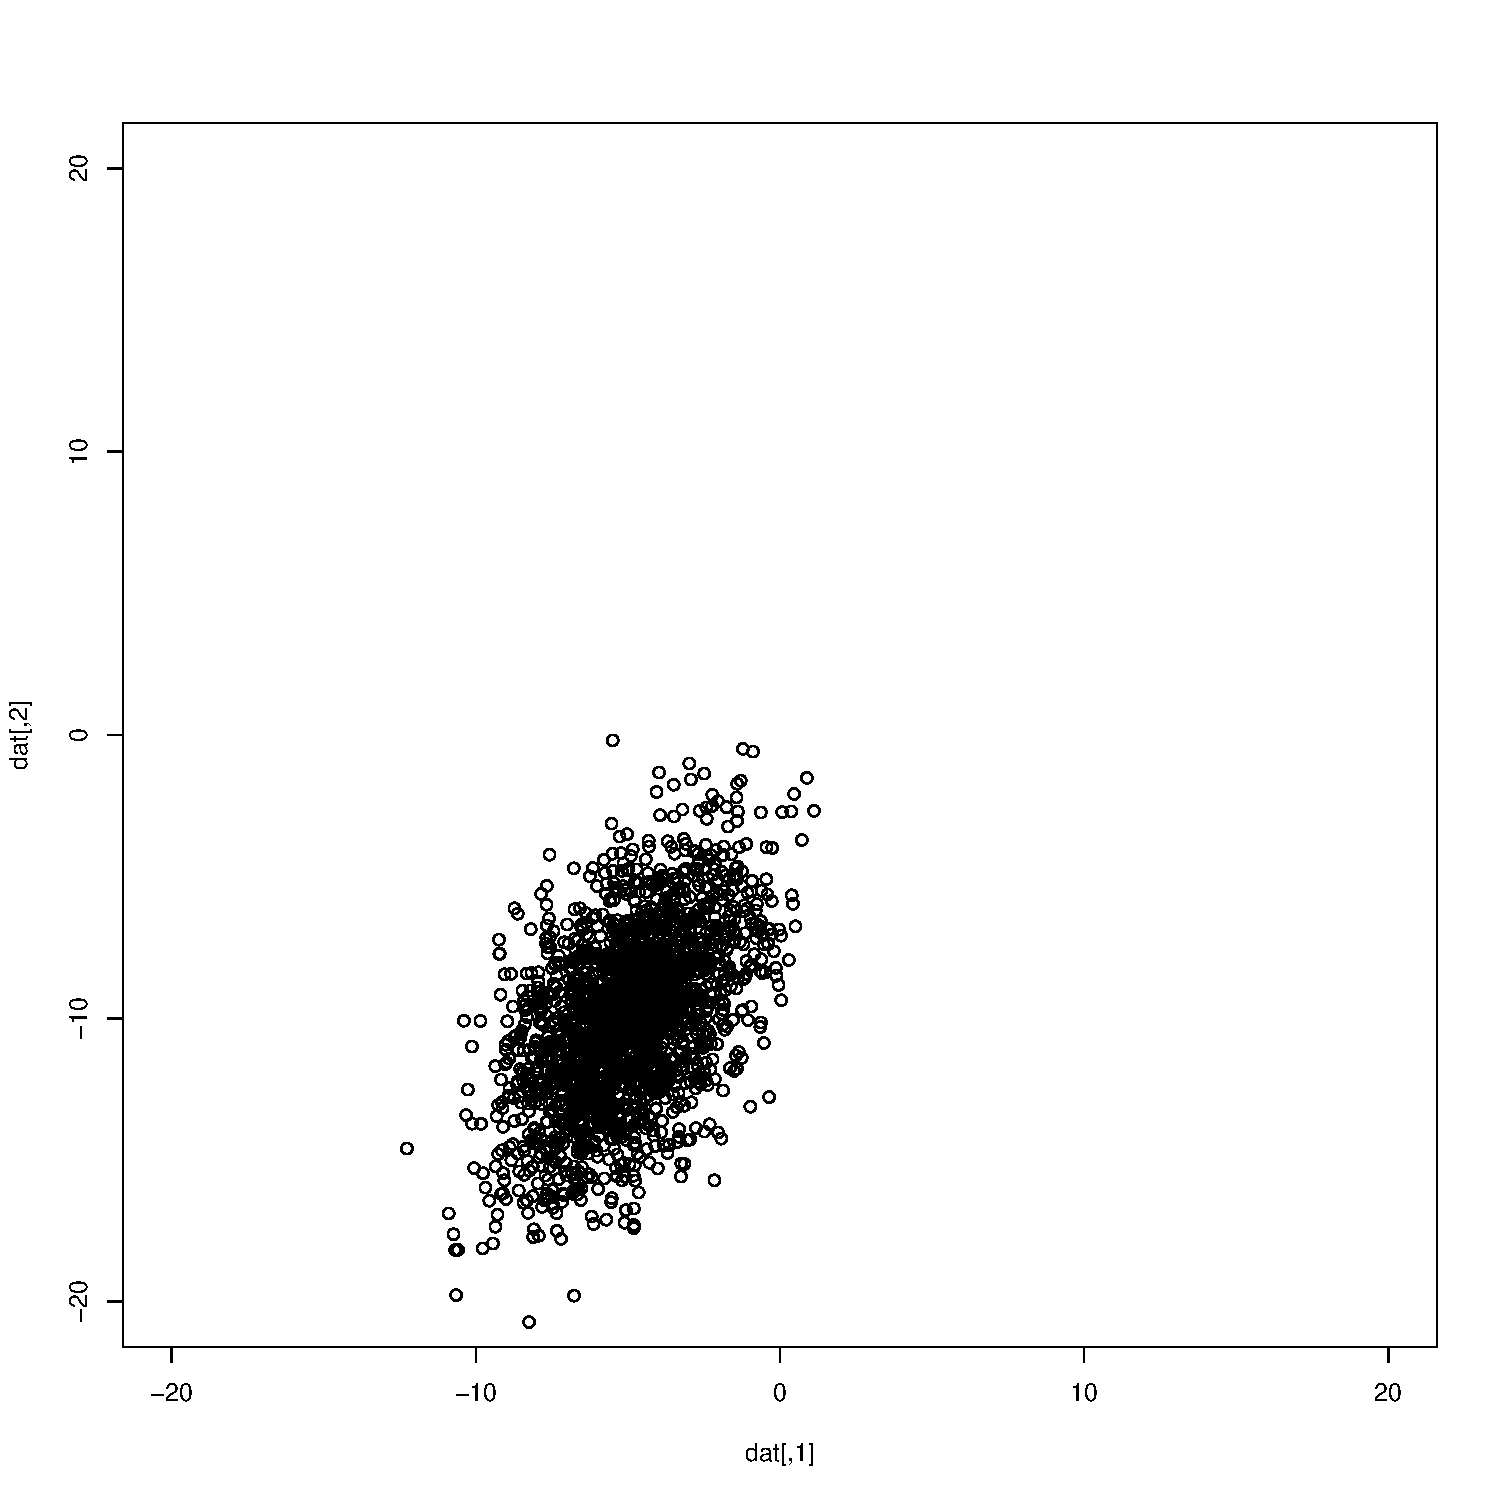
\includegraphics[width=\linewidth]{img/mvrnorm-plot1.pdf}
				\subcaption{第1項の正規分布}
				\label{img:mvrnorm-plot1}
			\end{minipage}
			\begin{minipage}{0.25\hsize}
				\centering
				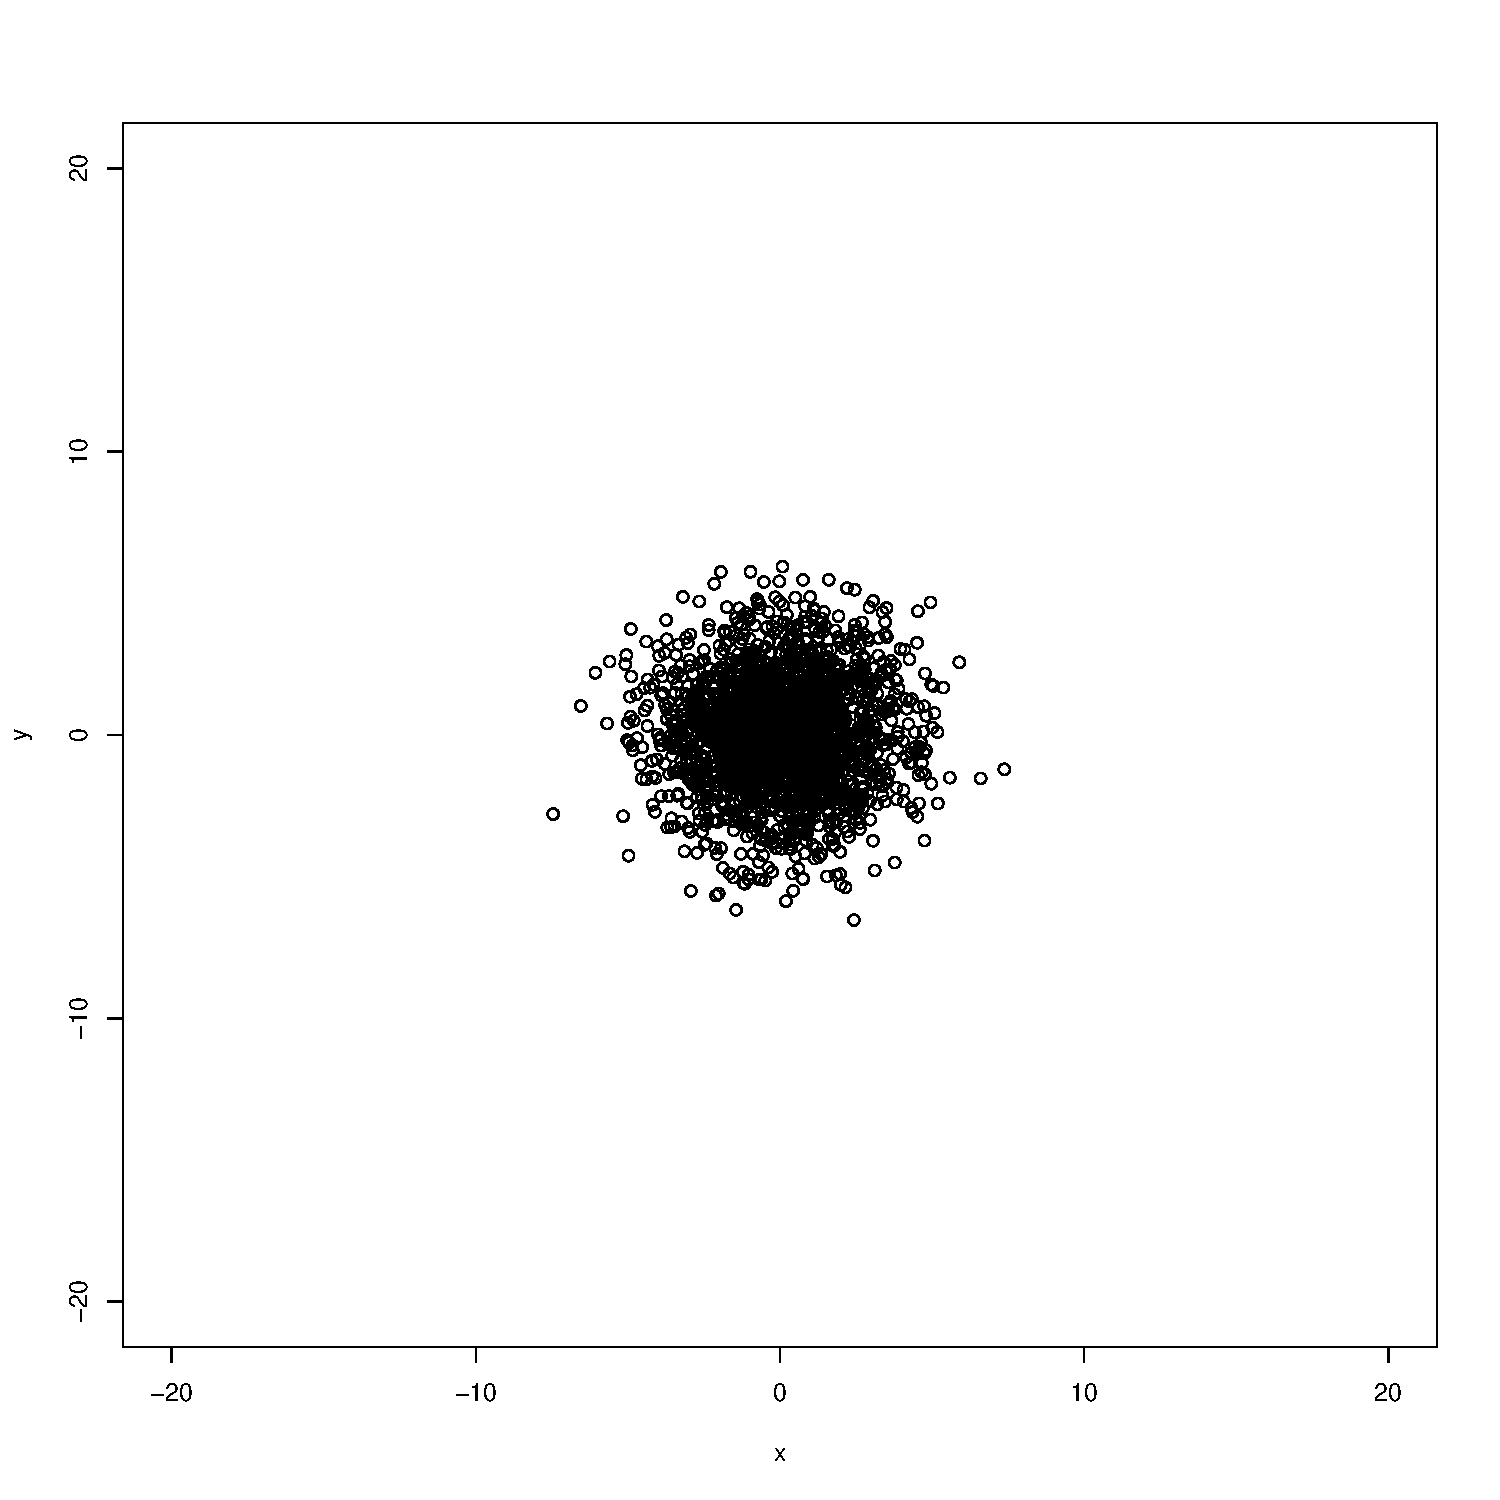
\includegraphics[width=\linewidth]{img/mvrnorm-plot2.pdf}
				\subcaption{第2項の正規分布}
				\label{img:mvrnorm-plot2}
			\end{minipage}
			\begin{minipage}{0.25\hsize}
				\centering
				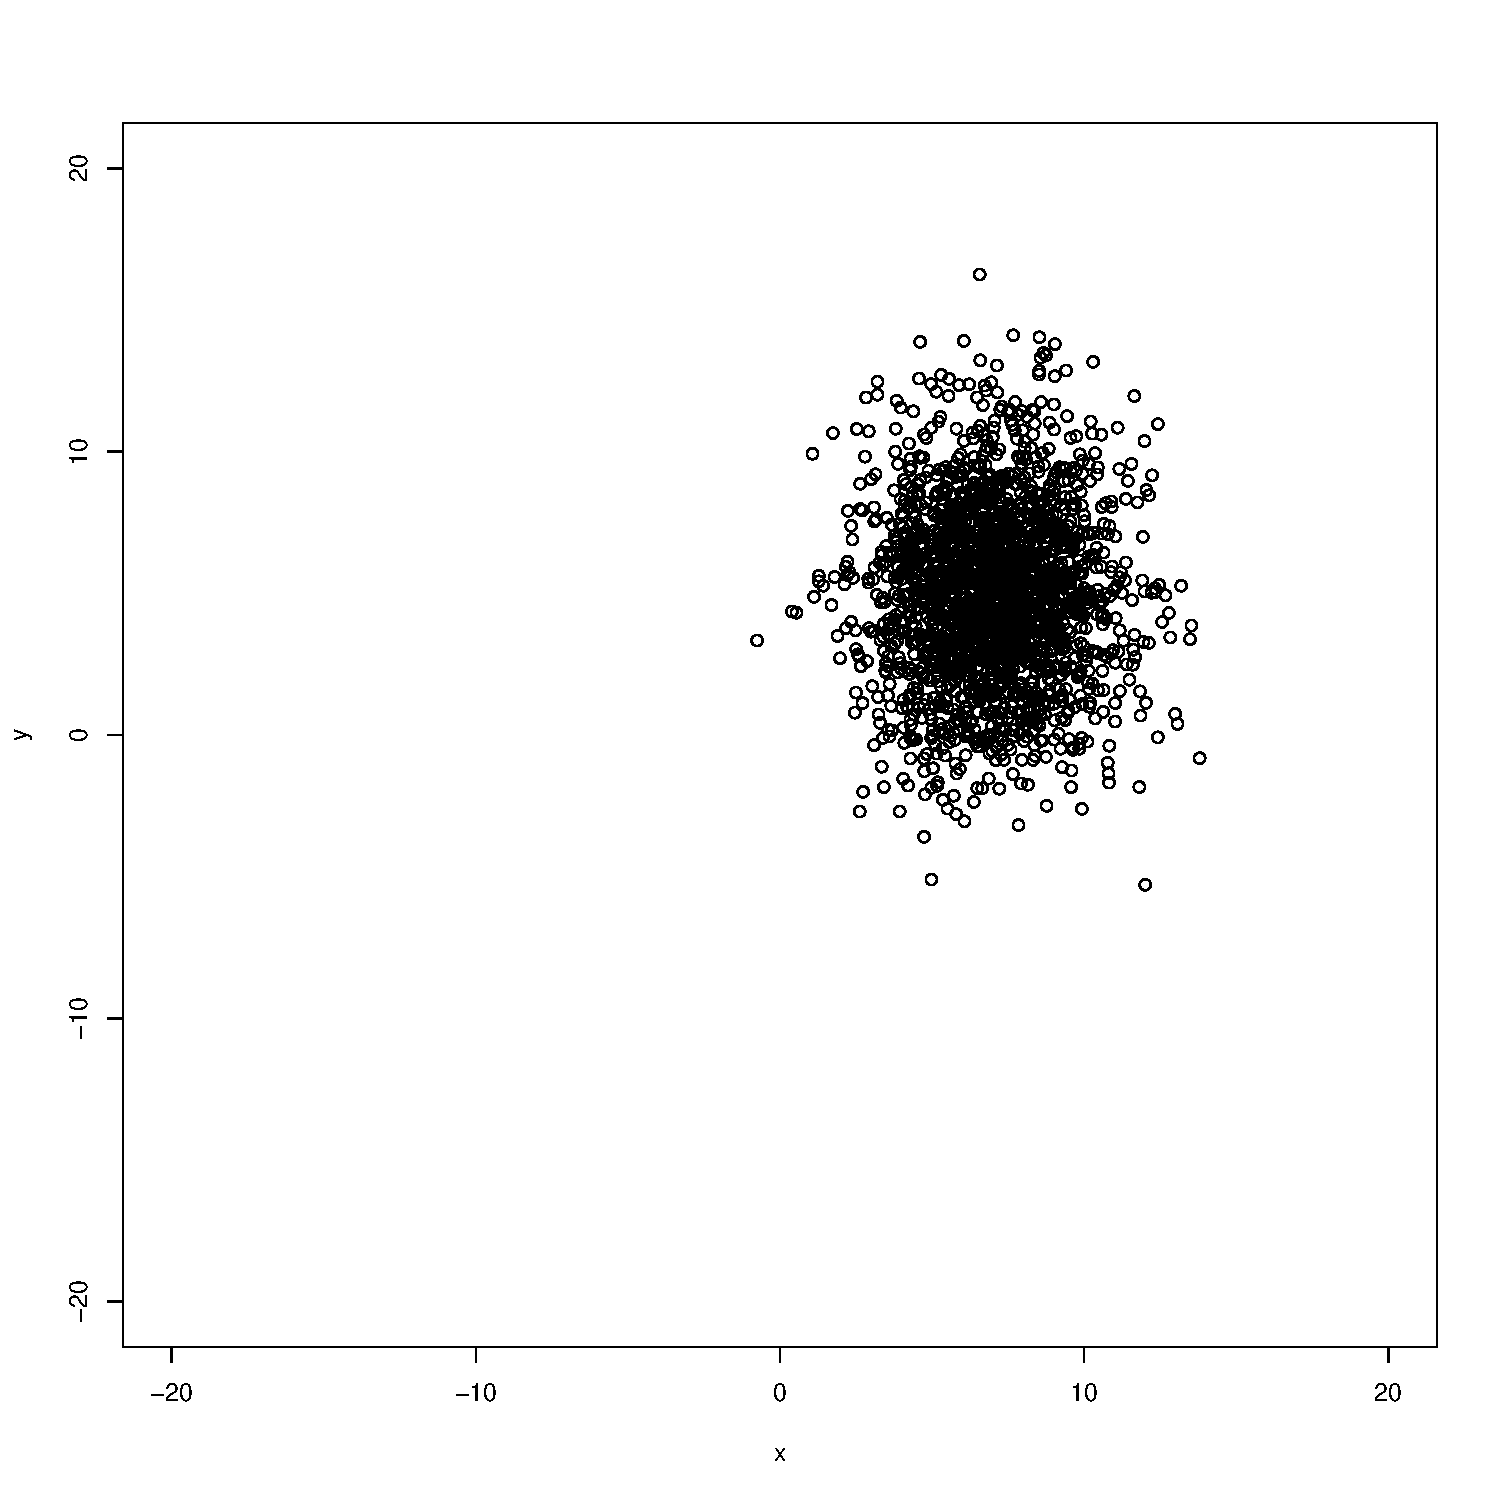
\includegraphics[width=\linewidth]{img/mvrnorm-plot3.pdf}
				\subcaption{第3項の正規分布}
				\label{img:mvrnorm-plot3}
			\end{minipage}
			\begin{minipage}{0.25\hsize}
				\centering
				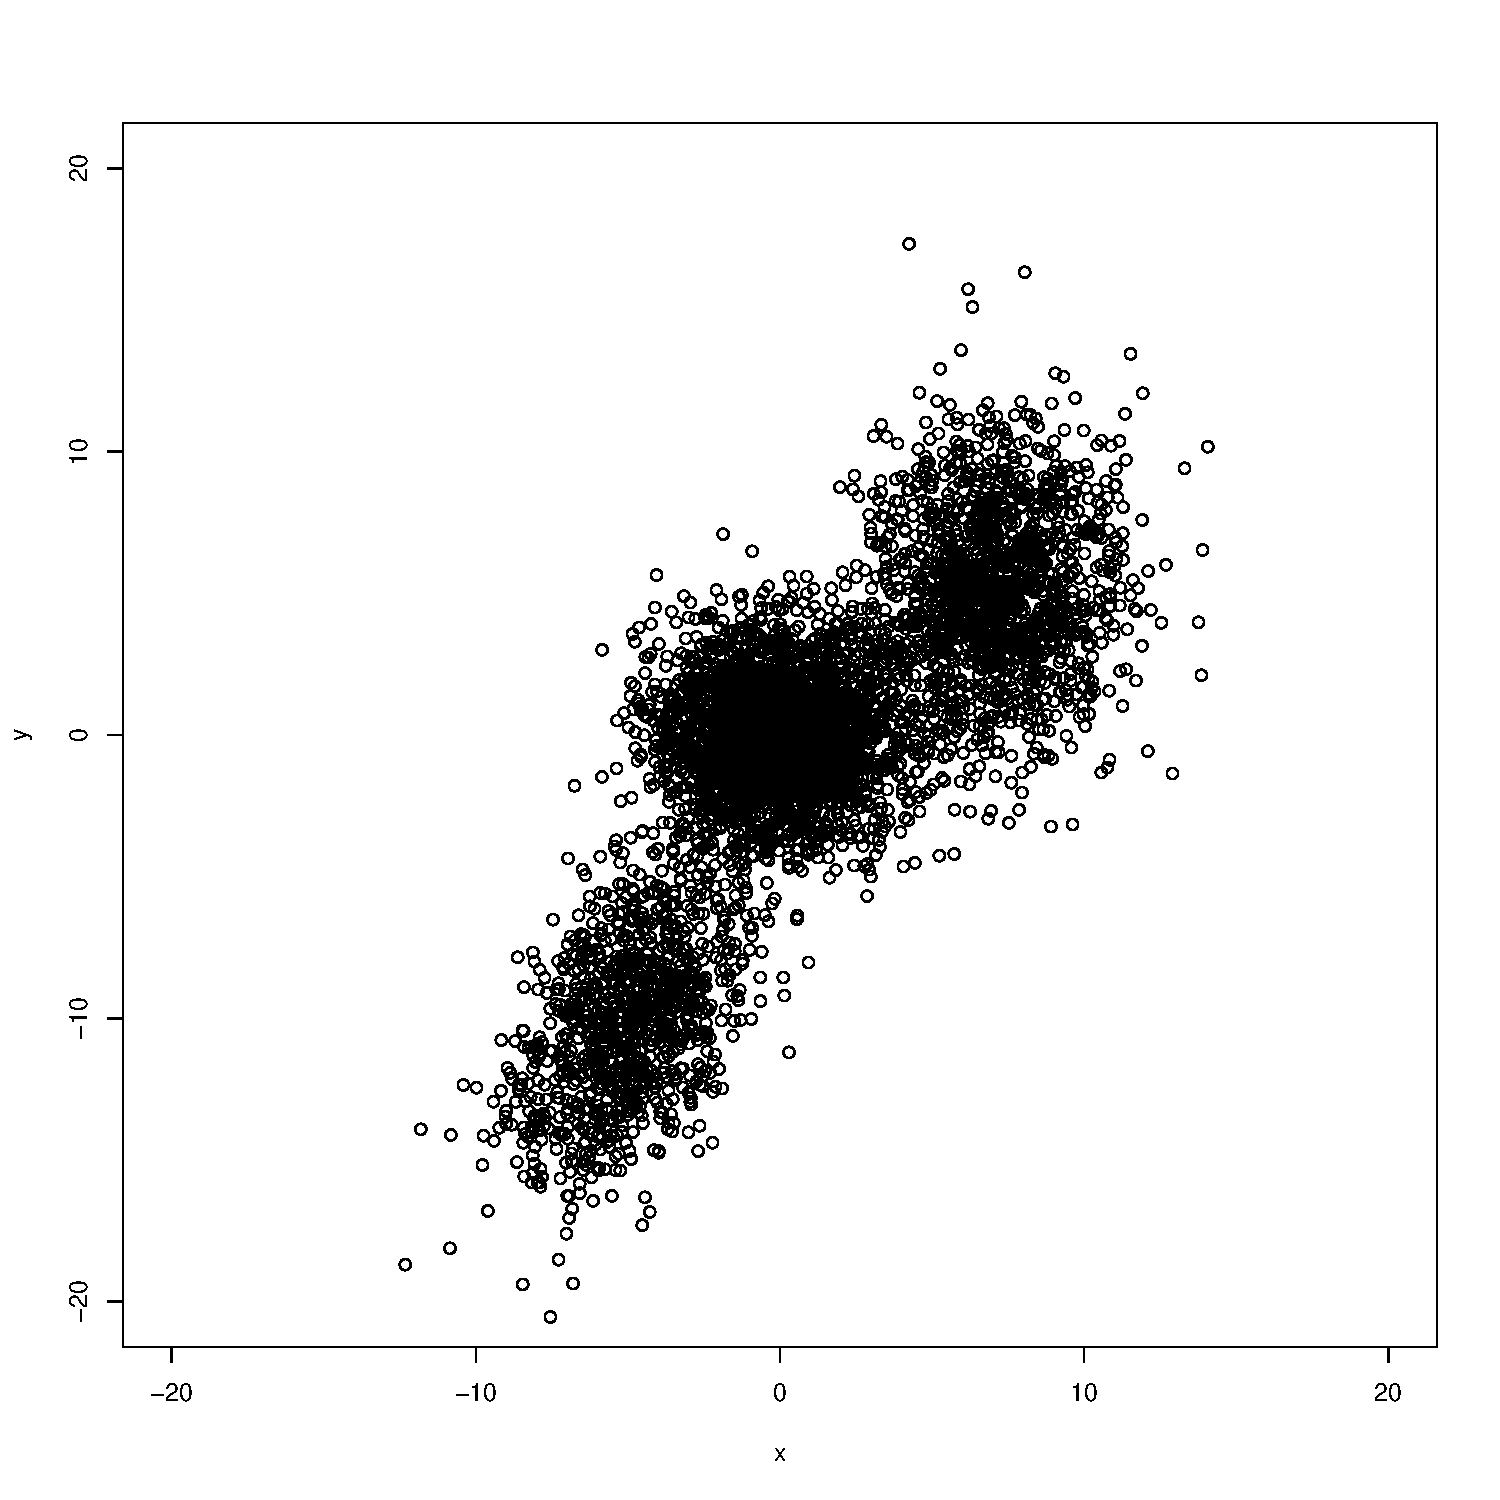
\includegraphics[width=\linewidth]{img/mvrnorm-plot.pdf}
				\subcaption{ガウス混合分布}
				\label{img:mvrnorm-plot-mix}
			\end{minipage}
		\end{tabular}
		\caption{生成乱数のプロット}
		\label{img:mvrnorm-plot}
	\end{minipage}
\end{figure}

\subsubsection*{考察}
図\ref{img:mvrnorm-plot}から,それぞれの分布が係数に合わせて
組み合わされていることが分かる.
密度は,係数が$0.5$の第2項が最も濃くなっており,
係数が$0.2$の第1項が最も薄くなっていることも確認できる.

\subsection*{7 EMアルゴリズム}
\subsubsection*{(1)}
6で作成した乱数ベクトル系列に対してEMアルゴリズムを適用し,
元の2変数3成分ガウス混合分布が推定できるか試してみよう.

\subsubsection*{スクリプト}
\begin{lstlisting}[basicstyle=\ttfamily\footnotesize, frame=single]
#install.packages("mclust")
library(mclust)

# 描画デバイスの作成
pdf("02\\mvrnorm-density.pdf", width=10, height=10)
dev = dev.cur()

# EMアルゴリズムの適用
res <- densityMclust(dat)

# プロット
dev.set(dev)
density(res, what="density", xlim=c(-20, 20), ylim=c(-20, 20))
dev.off(dev)

# 推測されたパラメータの確認
res$parameter$pro
res$parameter$mean
res$parameter$variance$sigma
\end{lstlisting}

\subsubsection*{結果}
それぞれの正規分布のみで生成した乱数に対しEMアルゴリズムを適用した結果を
図\ref{img:mvrnorm-density}
\subref{img:mvrnorm-density1}--\subref{img:mvrnorm-density3},
ガウス混合分布で生成した乱数に対しEMアルゴリズムを適用した結果を
図\ref{img:mvrnorm-density}\subref{img:mvrnorm-density-mix}
に示す.

\begin{figure}[b]
	\centering
	\begin{minipage}{0.8\hsize}
		\centering
		\begin{tabular}{c}
			\begin{minipage}{0.25\hsize}
				\centering
				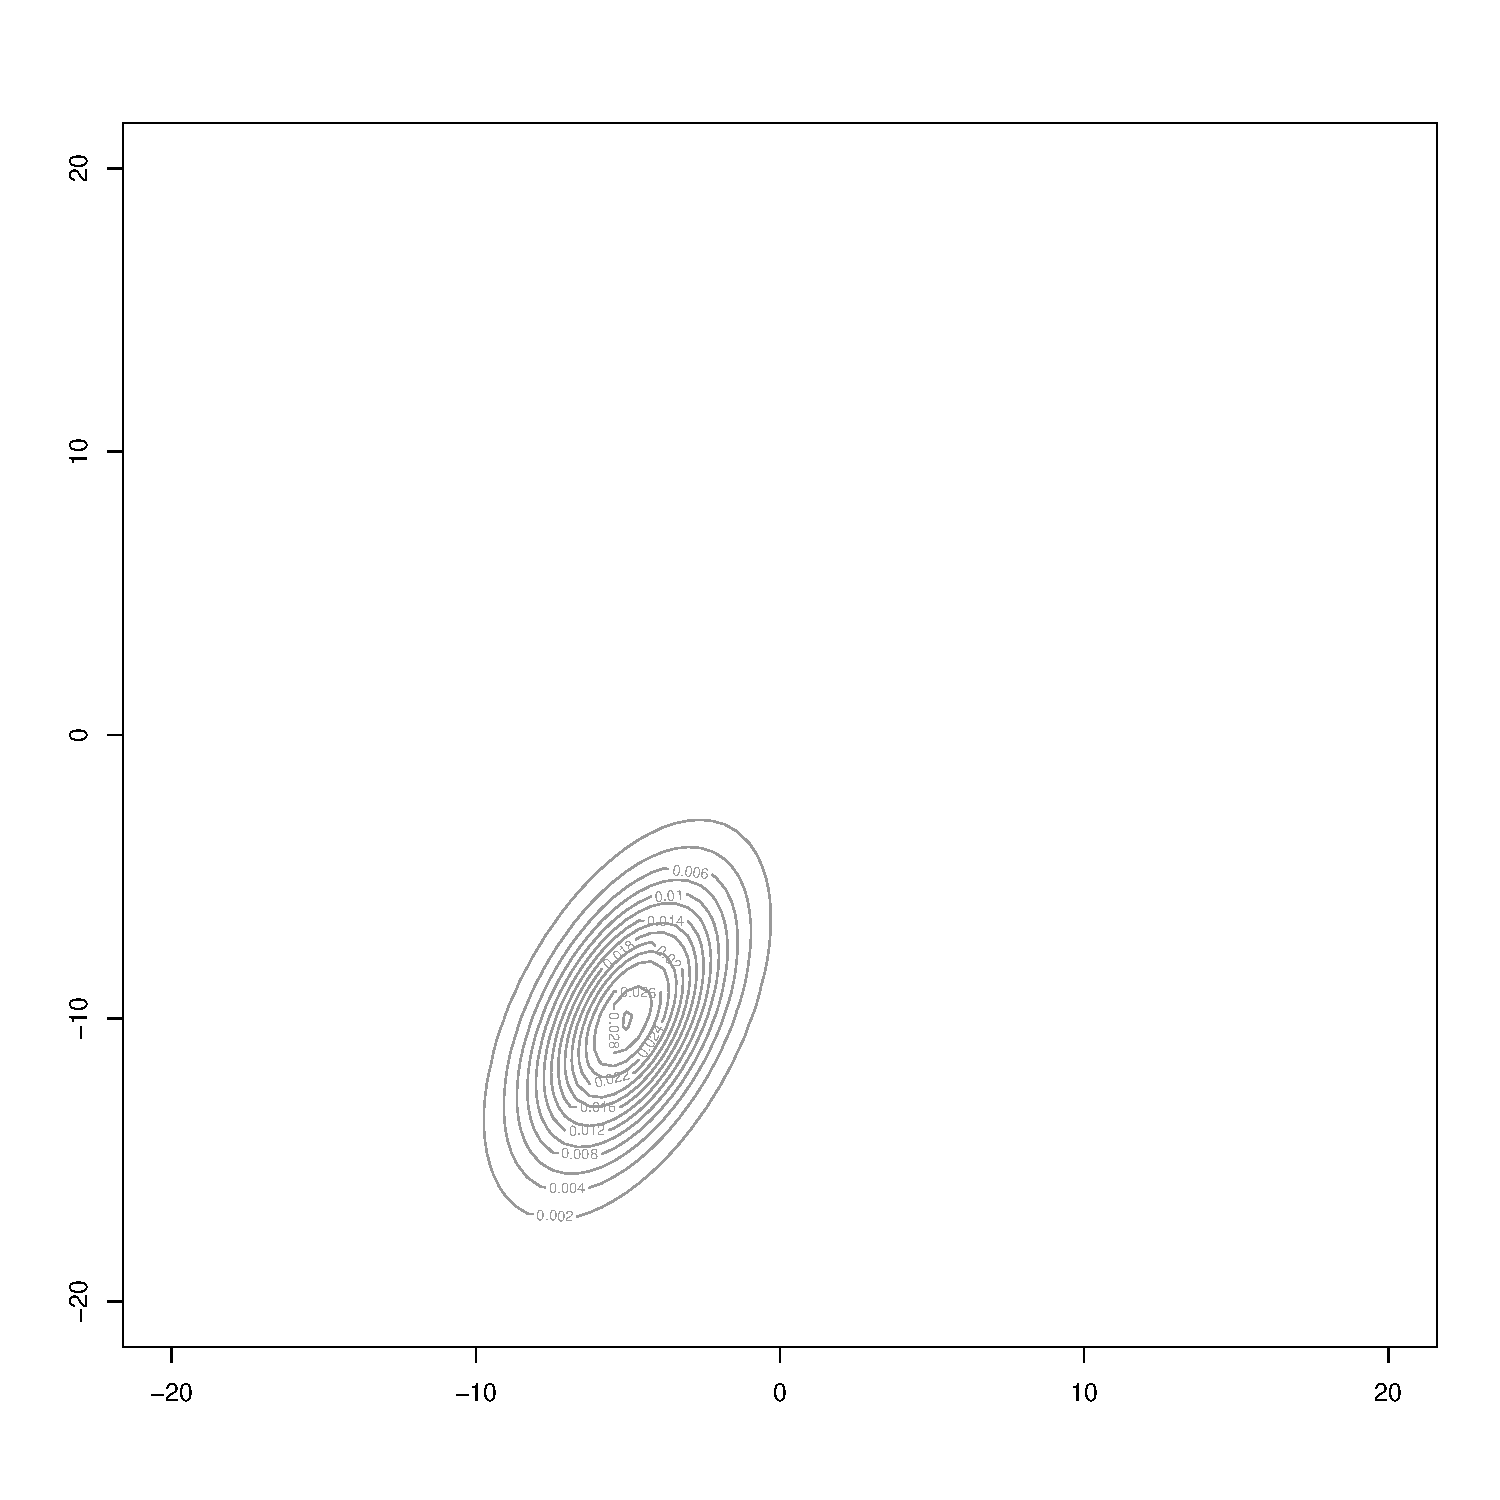
\includegraphics[width=\linewidth]{img/mvrnorm-density1.pdf}
				\subcaption{第1項の正規分布}
				\label{img:mvrnorm-density1}
			\end{minipage}
			\begin{minipage}{0.25\hsize}
				\centering
				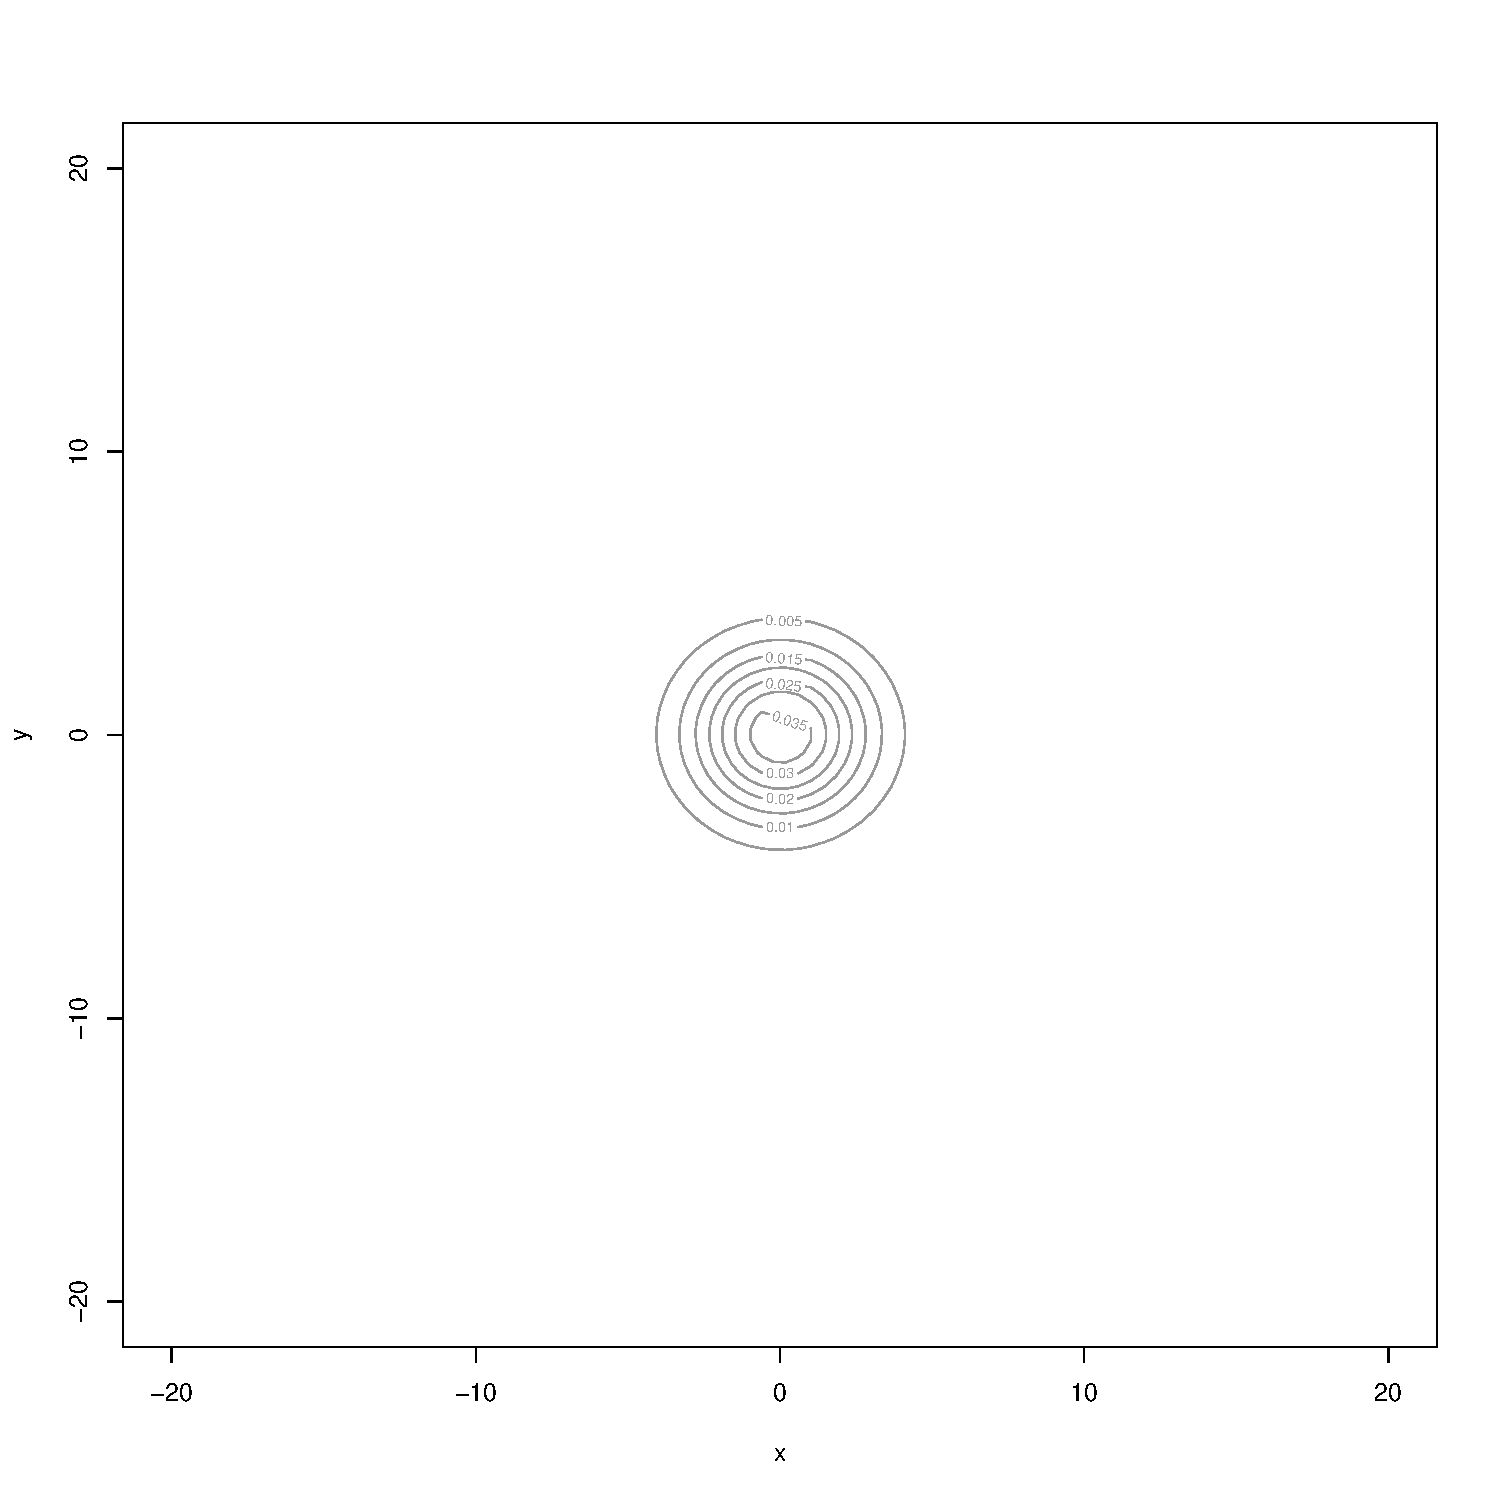
\includegraphics[width=\linewidth]{img/mvrnorm-density2.pdf}
				\subcaption{第2項の正規分布}
				\label{img:mvrnorm-density2}
			\end{minipage}
			\begin{minipage}{0.25\hsize}
				\centering
				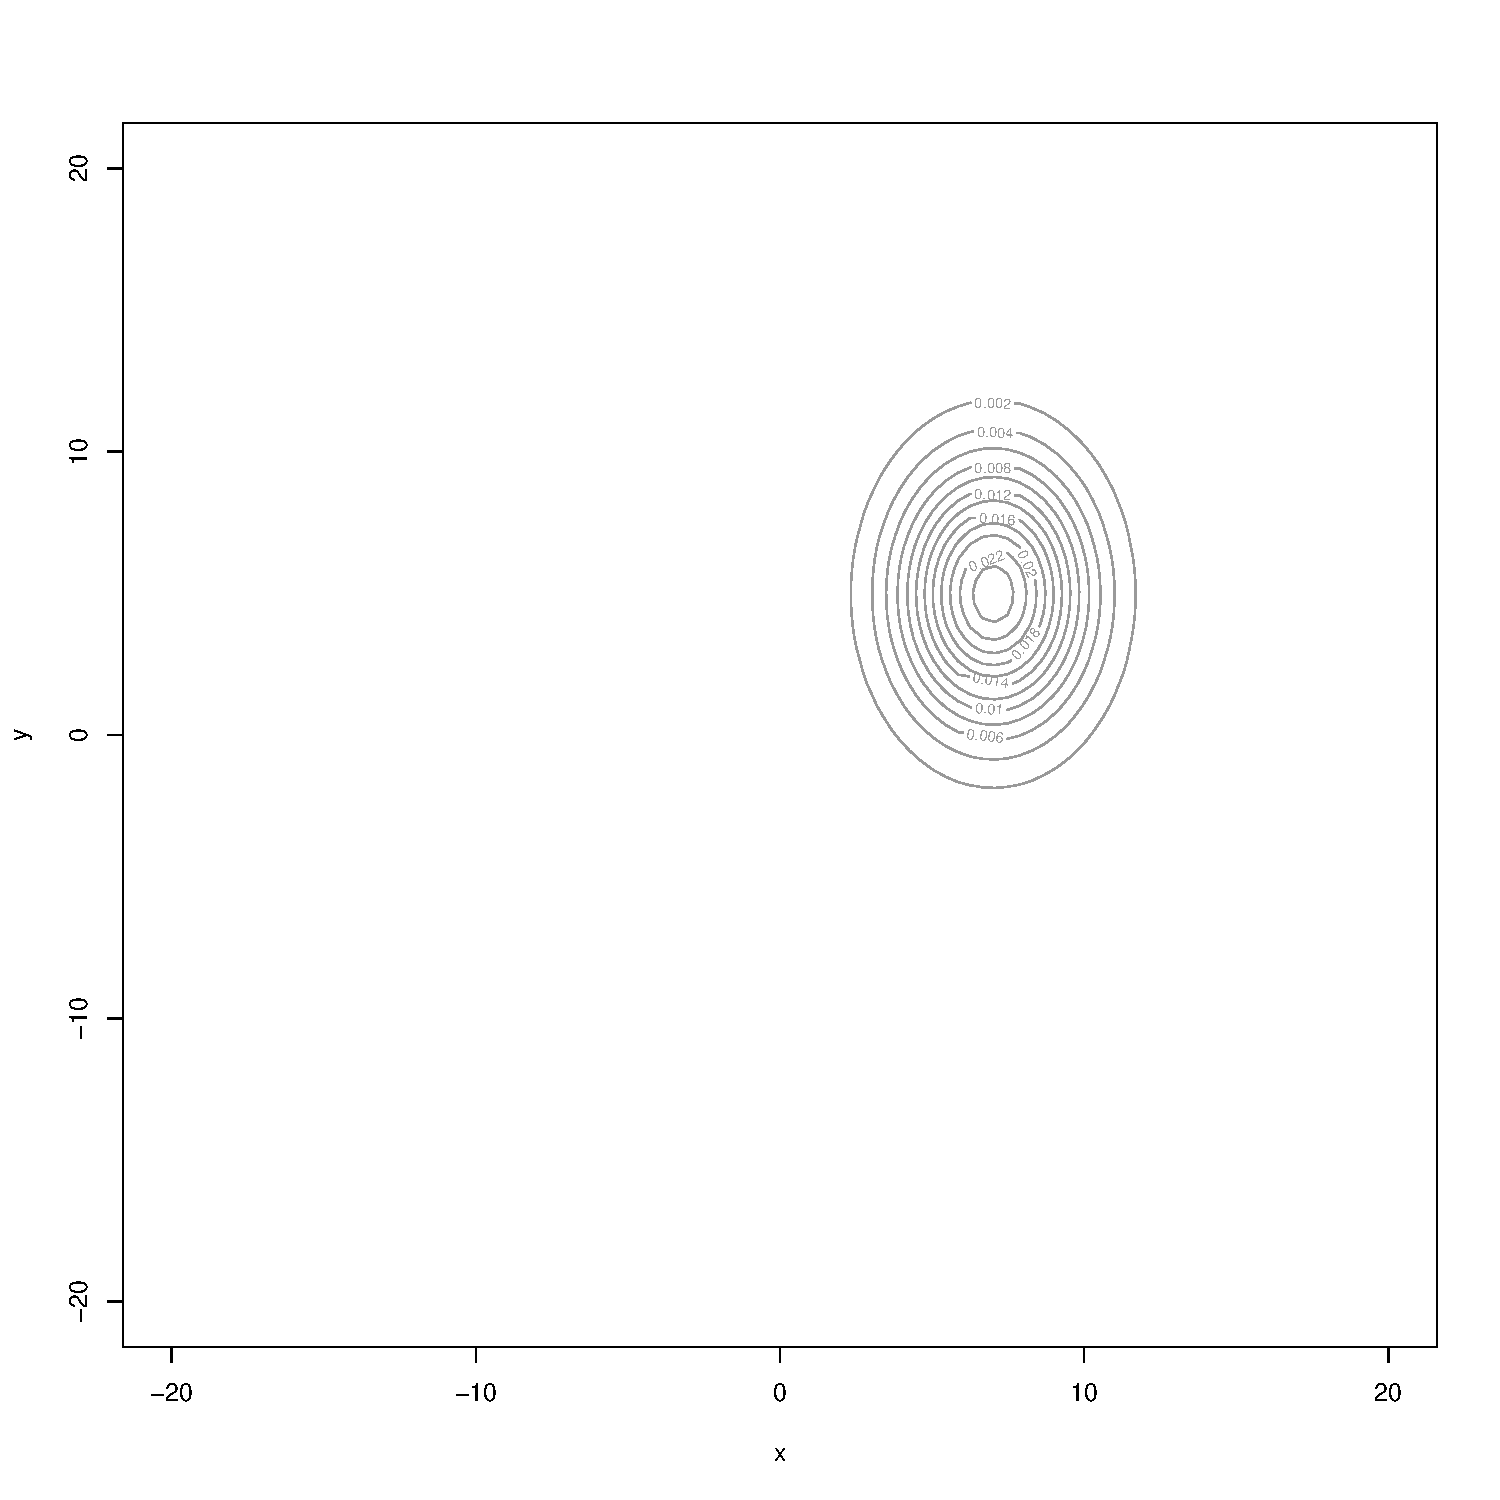
\includegraphics[width=\linewidth]{img/mvrnorm-density3.pdf}
				\subcaption{第3項の正規分布}
				\label{img:mvrnorm-density3}
			\end{minipage}
			\begin{minipage}{0.25\hsize}
				\centering
				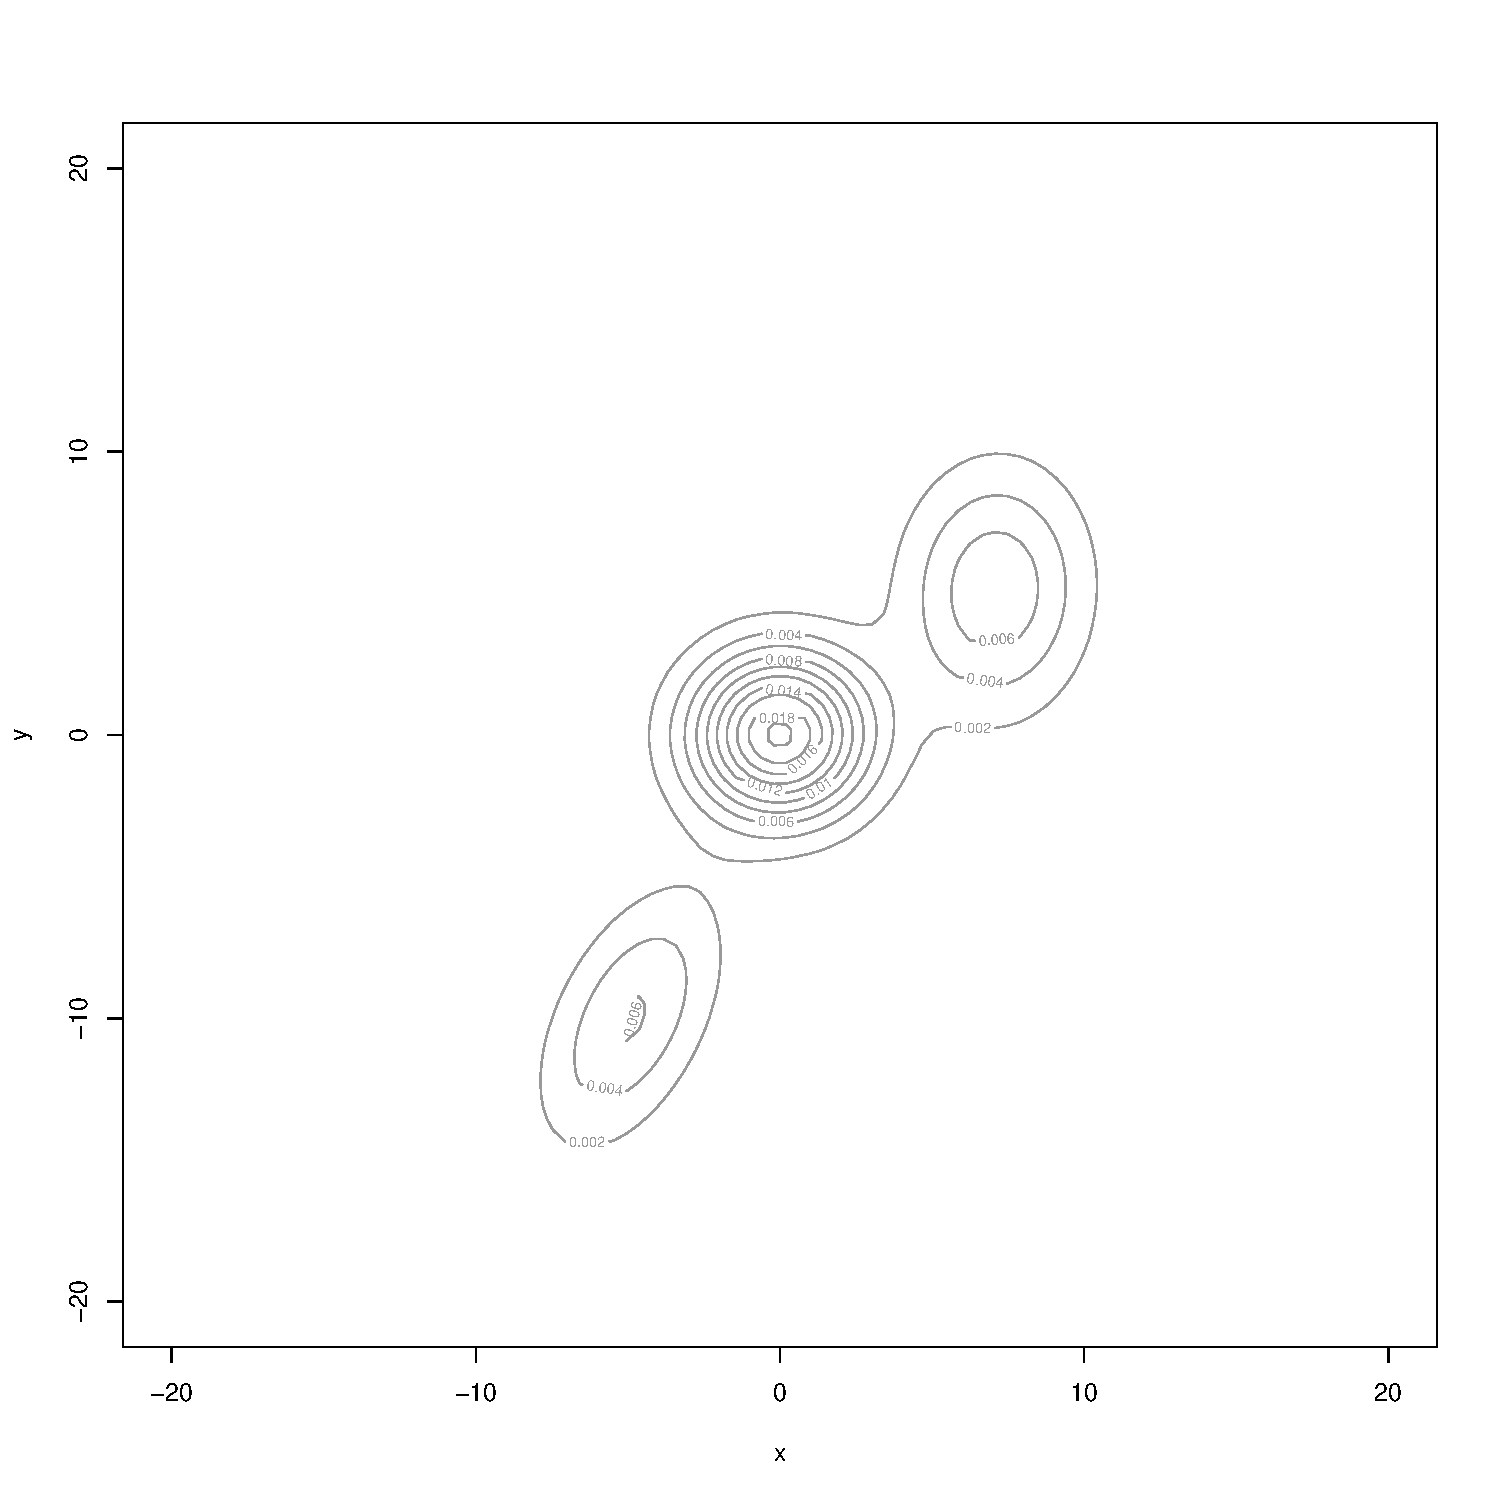
\includegraphics[width=\linewidth]{img/mvrnorm-density.pdf}
				\subcaption{ガウス混合分布}
				\label{img:mvrnorm-density-mix}
			\end{minipage}
		\end{tabular}
		\caption{生成乱数のプロット}
		\label{img:mvrnorm-density}
	\end{minipage}
\end{figure}

また,スクリプトの実行結果を以下に示す.
\begin{verbatim}
> res$parameter$pro
[1] 0.5087467 0.2898862 0.2013671
> res$parameter$mean
         [,1]     [,2]       [,3]
x -0.01517243 7.061727  -4.918003
y  0.01686892 5.102905 -10.013976
> res$parameter$variance$sigma
, , 1
           x          y
x 3.93317810 0.02366543
y 0.02366543 3.95526324

, , 2
          x         y
x 4.1815102 0.2287938
y 0.2287938 8.6670173

, , 3
         x        y
x 3.847105 2.898212
y 2.898212 9.065151
\end{verbatim}

\subsubsection*{考察}
図\ref{img:mvrnorm-plot}から,それぞれの分布が係数に合わせて
組み合わされていることが分かる.
密度関数の値は,係数が$0.5$の第2項が最も高くなっており,
係数が$0.2$の第1項が最も低くなっていることも確認できる.
また,第2項の等高線の間隔は狭く,
第1項,第3項の等高線の間隔が広くなっていることが確認できる.
このことから,元の2変数3成分ガウス混合分布が推定できたと考えられる.

推測されたパラメータは,係数の高い順に,第2項,第3項,第1項の順で
並んでいた.
推測された係数は,順に$0.509, 0.290, 0.201$となり,
設定した$0.5, 0.3, 0.2$と一致している.
また,平均$\mu$,分散共分散行列$\Sigma$についても式\ref{eqn:parameters}
で設定した値と概ね一致していた.

\subsection*{10 区間推定}
\subsubsection*{(1)}
\verb|rnorm(N, mean=0.86, sd=1.3)|から生成される乱数集合を用いて
その平均値の$95\%$信頼区間が,\verb|N|の変化によってどう変わるか,
グラフに示してみよう.
また,この乱数集合の分散の信頼区間についても同様に示してみよう.

\subsubsection*{スクリプト}
\begin{lstlisting}[basicstyle=\ttfamily\footnotesize, frame=single]
f <- function(max) {
  sdkn <- c() # 既知の標準偏差を用いた信頼区間 (正規分布)
  sdun <- c() # 推定標準偏差を用いた信頼区間 (正規分布)
  sdkt <- c() # 既知の標準偏差を用いた信頼区間 (t分布)
  sdut <- c() # 推定標準偏差を用いた信頼区間 (t分布)
  vux <- c() # 不偏分散を用いた区間推定 (カイ二乗分布)

  for(N in 2:max) {
    # 初期化
    dat <- rnorm(N, mean=0.86, sd=1.3)
    mu <- mean(dat); sigma <- sd(dat)

    # 平均値の区間推定
    sdkn <- rbind(sdkn, (qnorm(c(0.025, 0.975)) * 1.3 / sqrt(N) + mu))
    sdun <- rbind(sdun, (qnorm(c(0.025, 0.975)) * sigma /  sqrt(N) + mu))
    sdkt <- rbind(sdkt, (qt(c(0.025, 0.975), df=(N-1)) * 1.3 / sqrt(N) + mu))
    sdut <- rbind(sdut, (qt(c(0.025, 0.975), df=(N-1)) * sigma /  sqrt(N) + mu))
    # 分散の区間推定
    vux <- rbind(vux, ((N-1) * sigma**2 / qchisq(c(0.975, 0.025), df=(N-1))))
  }

  res <- list(sdkn, sdun, sdkt, sdut, vux)
  return(res)
}

# グラフの保存
save <- function(res){
  for(i in 1:length(names)) {
    pdf(sprintf("02\\%s-%d.pdf", names[i], N), width=10, height=10)
    devnum = dev.cur()
  
    a = res[[i]]
  
    dev.set(devnum)
    plot(0, 0, type = "n", xlab = "N", ylab = names[i],
      xlim=c(0, N), ylim=c(tv[i]-2, tv[i]+2))
    lines(2:N-1, a[,1], col="red"); lines(2:N-1, a[,2], col="red")
    lines(c(0, N-1), c(tv[i], tv[i]), col="green4")
    dev.off(devnum)
  }
}

names <- c("sdkn", "sdun", "sdkt", "sdut", "vux")
tv <- c(0.86, 0.86, 0.86, 0.86, 1.3**2)
N <- 500; res <- f(N); save(res)
\end{lstlisting}

\subsubsection*{結果}
データ数$N$を変化させながら,
平均$\mu$を区間推定した結果を図\ref{img:estimate-mean}に,
分散$\sigma^2$を区間推定した結果を図\ref{img:estimate-variance}に示す.
グラフの横軸は$N$,縦軸は値である.
上の赤線が推定区間の上の値を,
下の赤線が推定区間の下の値を,
緑の直線が母集団の平均,および分散を示す.

\subsubsection*{考察}
図\ref{img:estimate-mean}, \ref{img:estimate-variance}から,
発生した乱数によって推定区間が大きく変動することが確認できる.
そこで,上記のスクリプトを$10000$回実行し,推定区間の値を平均することで,
乱数による影響を抑えたグラフを作成した
(図\ref{img:estimate-mean-mean}, \ref{img:estimate-variance-mean}).

図\ref{img:estimate-mean-mean}, \ref{img:estimate-variance-mean}より,
平均,分散共に95\%信頼区間はデータ数$N$を増やすほど
狭くなっていることが分かる.
したがって,$N$を増やすほど推定の精度が上がることが分かる.

平均の区間推定においては,$N=200$程度から大きく差が出ないことが
確認できる.
正規分布を用いて区間推定を行った場合
(図\ref{img:estimate-mean-mean}\subref{img:sdkn-mean})と,
\emph{t}分布を用いて区間推定を行った場合
(図\ref{img:estimate-mean-mean}\subref{img:sdkt-mean})を比較すると,
$N$が小さいときは正規分布では推定区間が非常に大きく,精度が低いが,
\emph{t}分布では推定区間が狭く,比較的精度が高いことが分かる.
既知の標準偏差を用いた場合
(図\ref{img:estimate-mean-mean}\subref{img:sdkt-mean},
\subref{img:sdkn-mean}) と推定標準偏差を用いた場合
(図\ref{img:estimate-mean-mean}\subref{img:sdut-mean},
\subref{img:sdun-mean}) の間には大きな差はないと考える.
よって,データの標準偏差が既知でない場合でも,
同等な区間推定ができると考えられる.

また,図\ref{img:estimate-mean-mean}に比べ,
図\ref{img:estimate-variance-mean}は
$N$が小さいときの推定区間が広く,その後もなかなか推定区間が狭くならない.
このことから,分散の区間推定においては,推定の精度を高くするためには,
平均の区間推定よりも多くのデータ数が必要であると考えられる.

\begin{figure}[b]
	\centering
	\begin{minipage}{\hsize}
		\centering
		\begin{tabular}{c}
			\begin{minipage}{0.25\hsize}
				\centering
				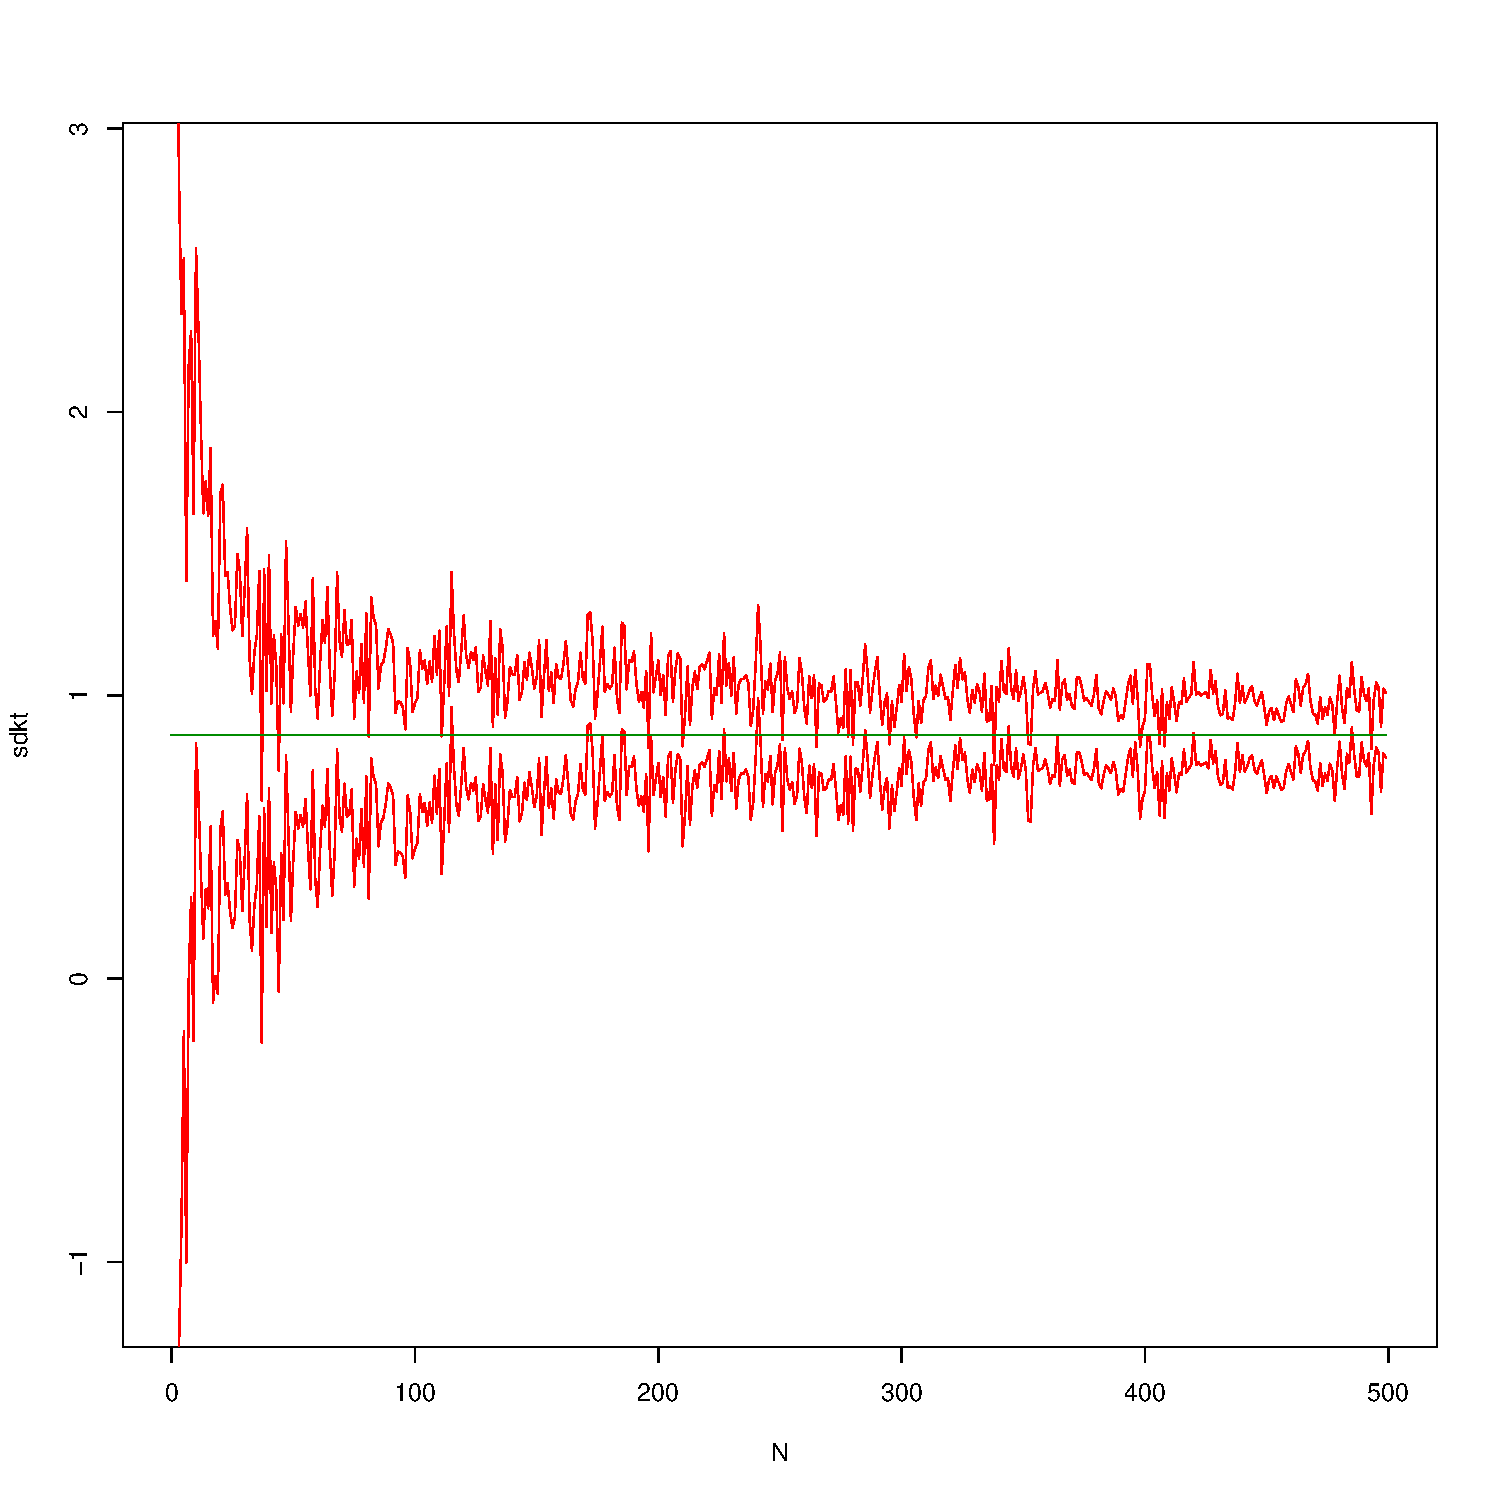
\includegraphics[width=\linewidth]{img/sdkt-500.pdf}
				\subcaption{既知の標準偏差使用\\(\emph{t}分布)}
				\label{img:sdkt}
			\end{minipage}
			\begin{minipage}{0.25\hsize}
				\centering
				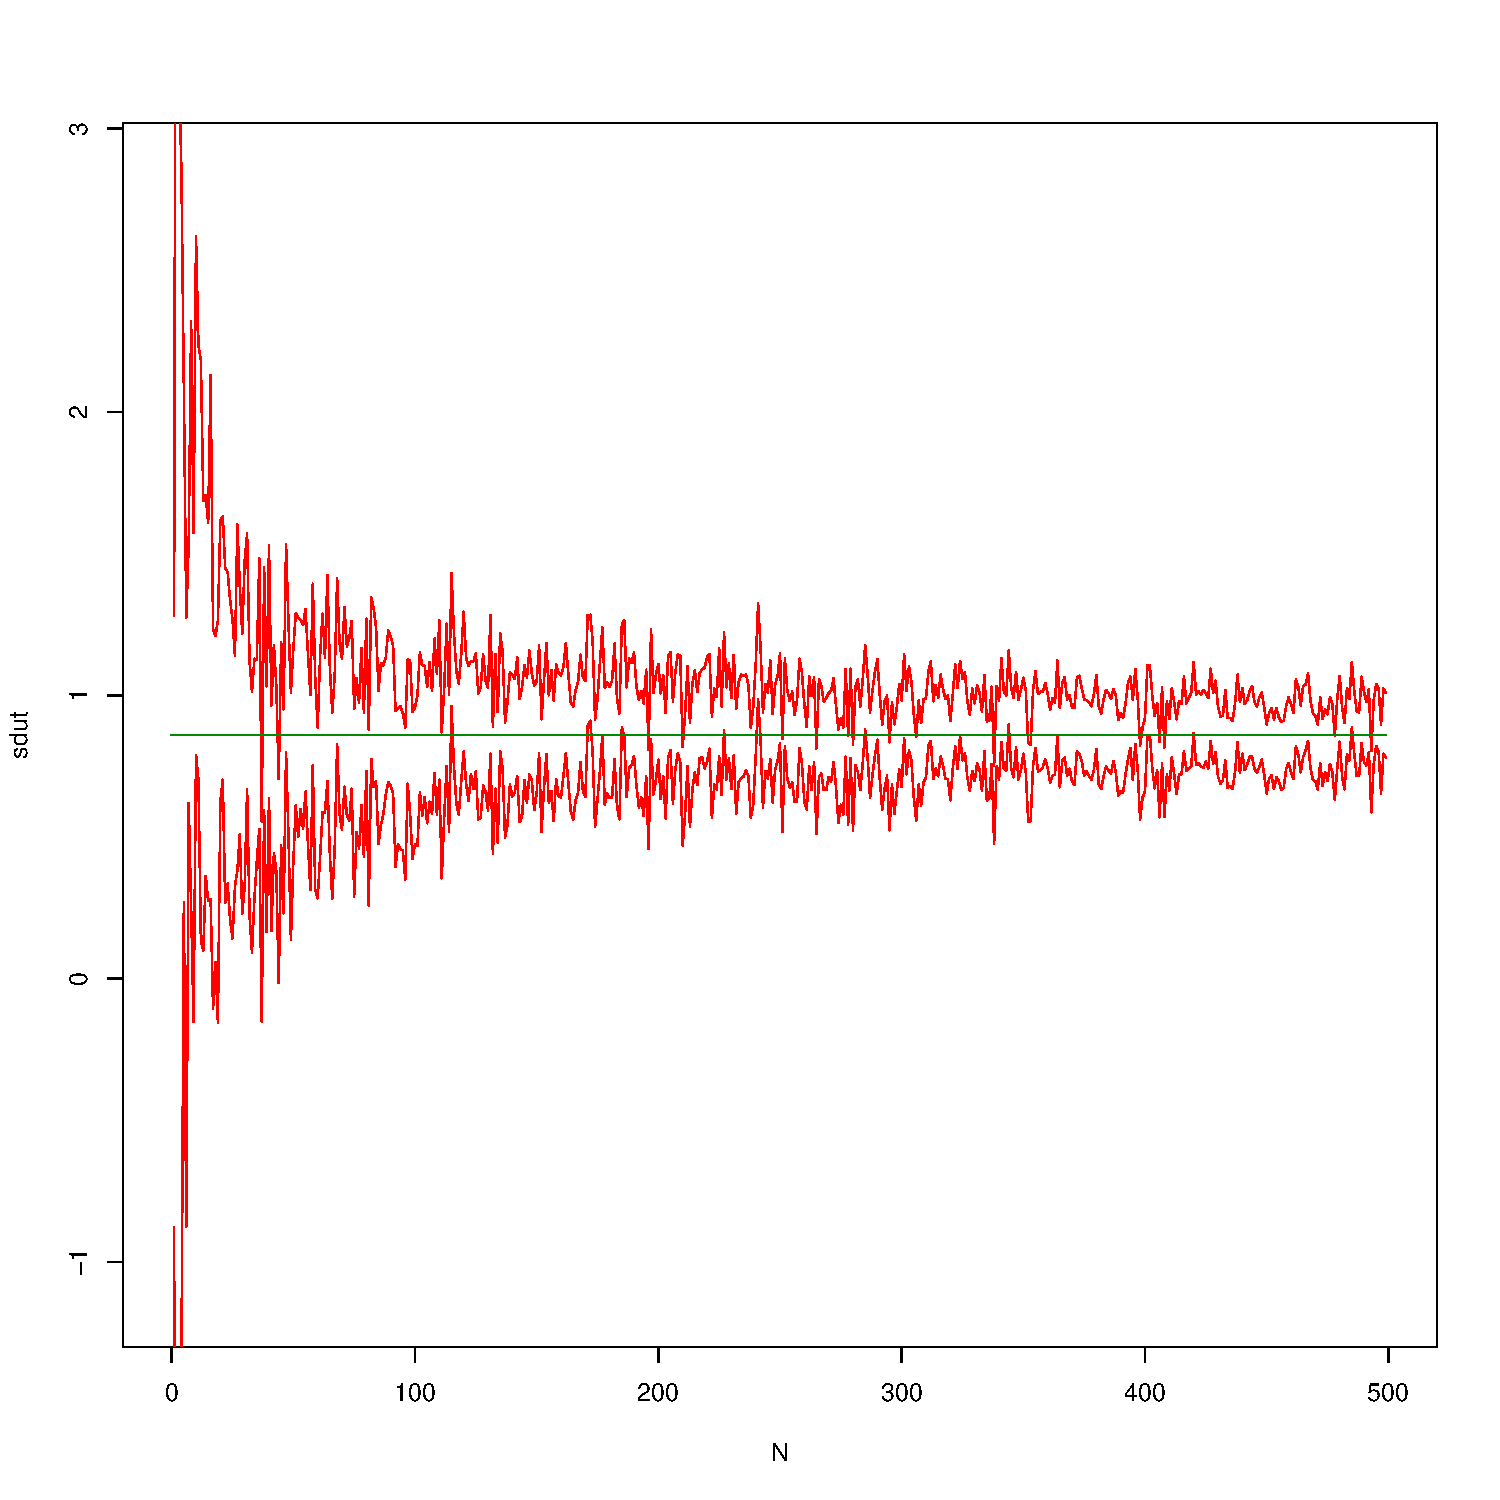
\includegraphics[width=\linewidth]{img/sdut-500.pdf}
				\subcaption{推定標準偏差使用\\(\emph{t}分布)}
				\label{img:sdut}
			\end{minipage}
			\begin{minipage}{0.25\hsize}
				\centering
				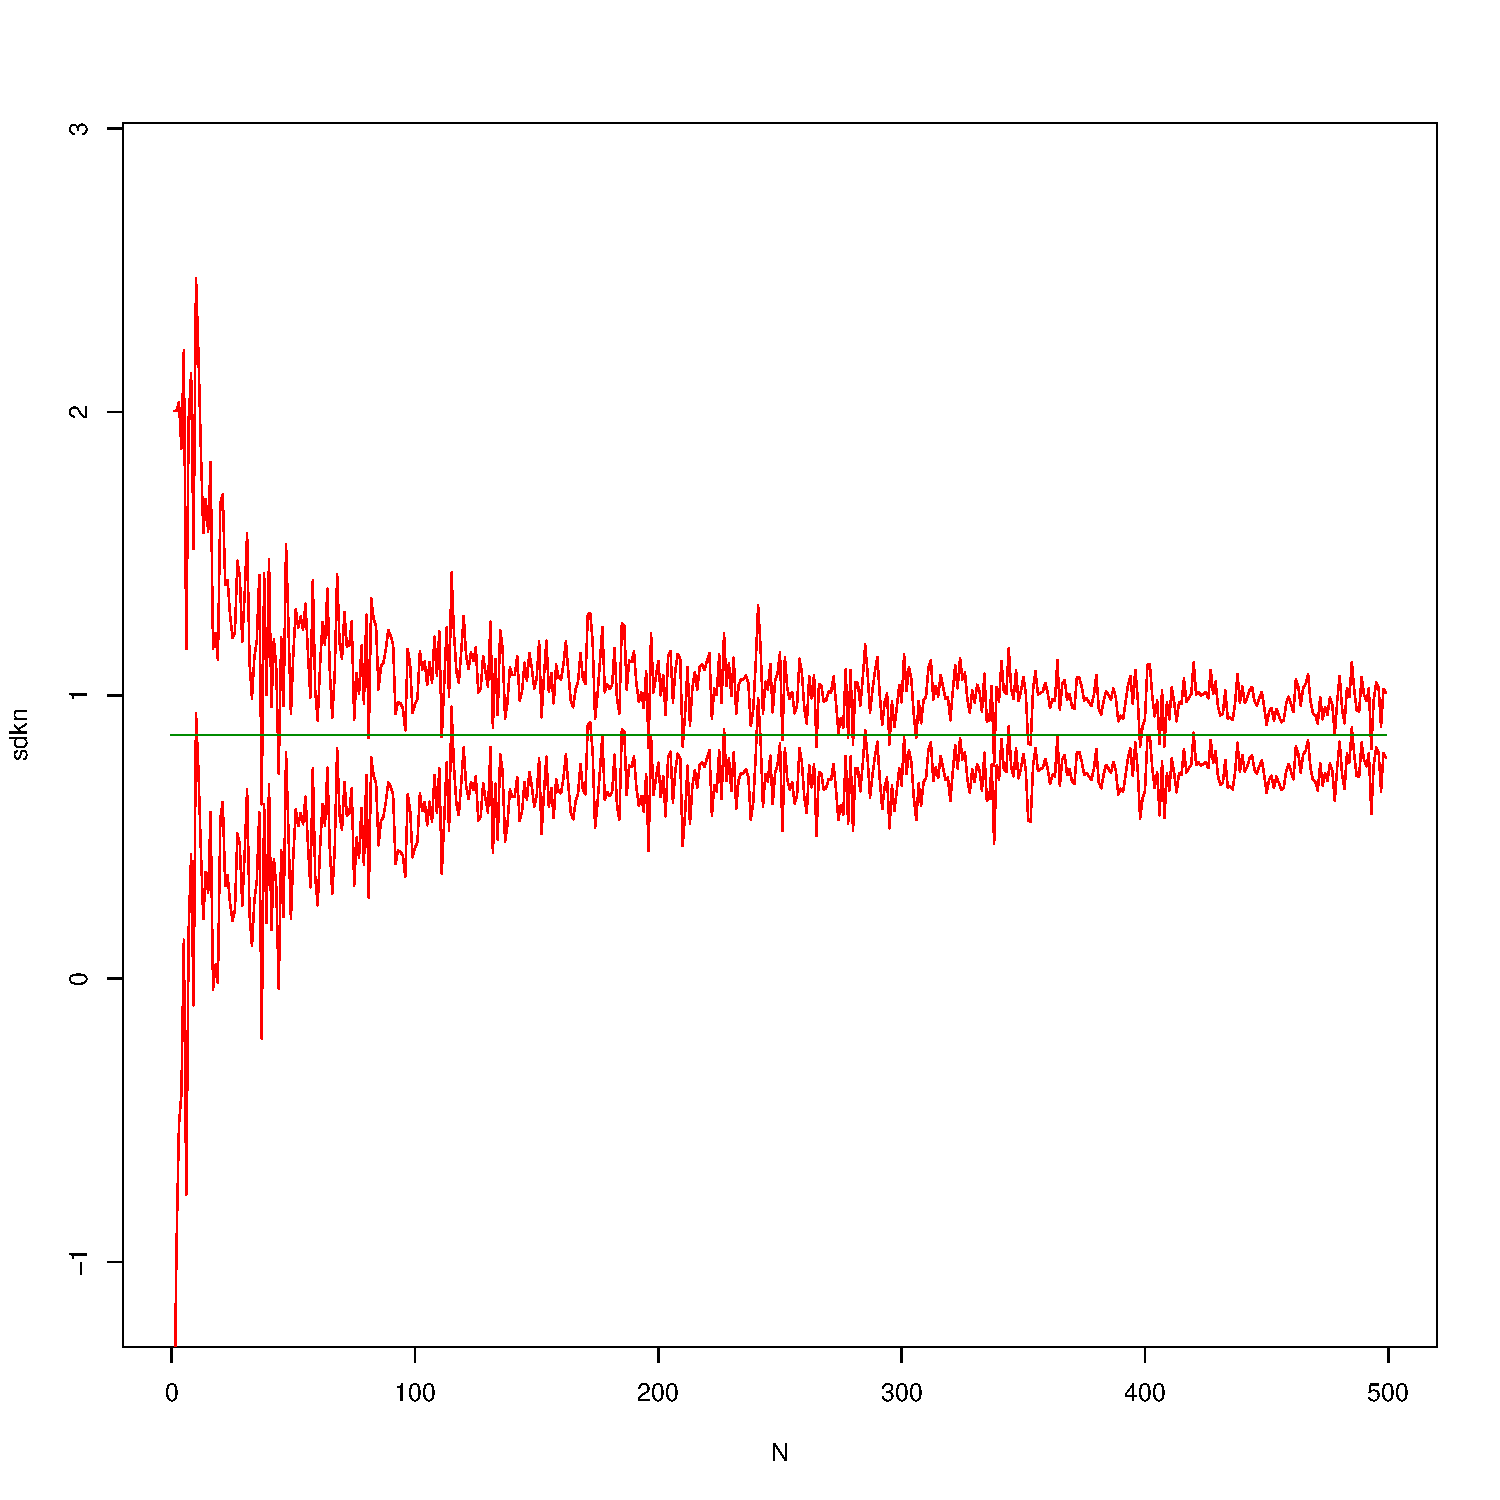
\includegraphics[width=\linewidth]{img/sdkn-500.pdf}
				\subcaption{既知の標準偏差使用\\(正規分布)}
				\label{img:sdkn}
			\end{minipage}
			\begin{minipage}{0.25\hsize}
				\centering
				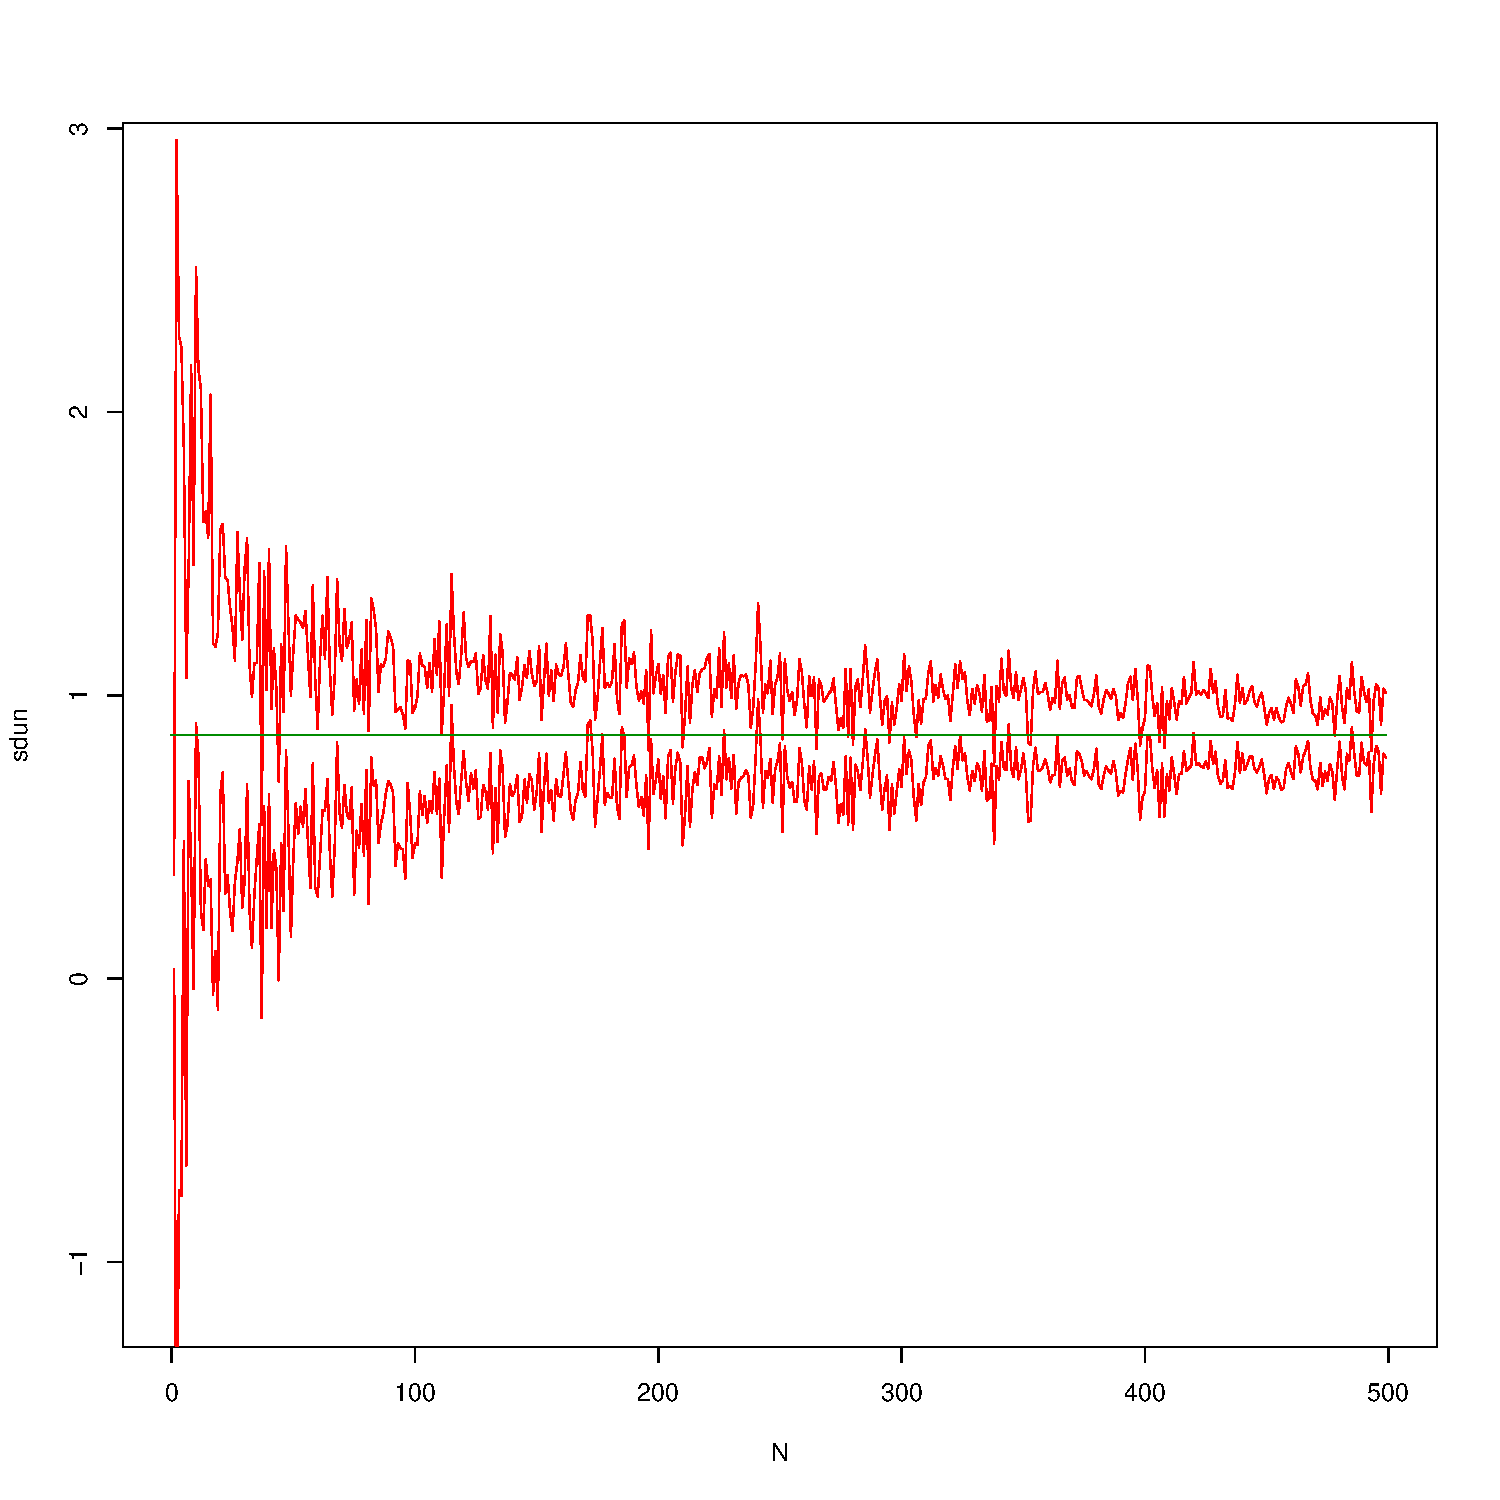
\includegraphics[width=\linewidth]{img/sdun-500.pdf}
				\subcaption{推定標準偏差使用\\(正規分布)}
				\label{img:sdun}
			\end{minipage}
		\end{tabular}
		\caption{平均の区間推定 (95\%信頼区間)}
		\label{img:estimate-mean}
	\end{minipage}
	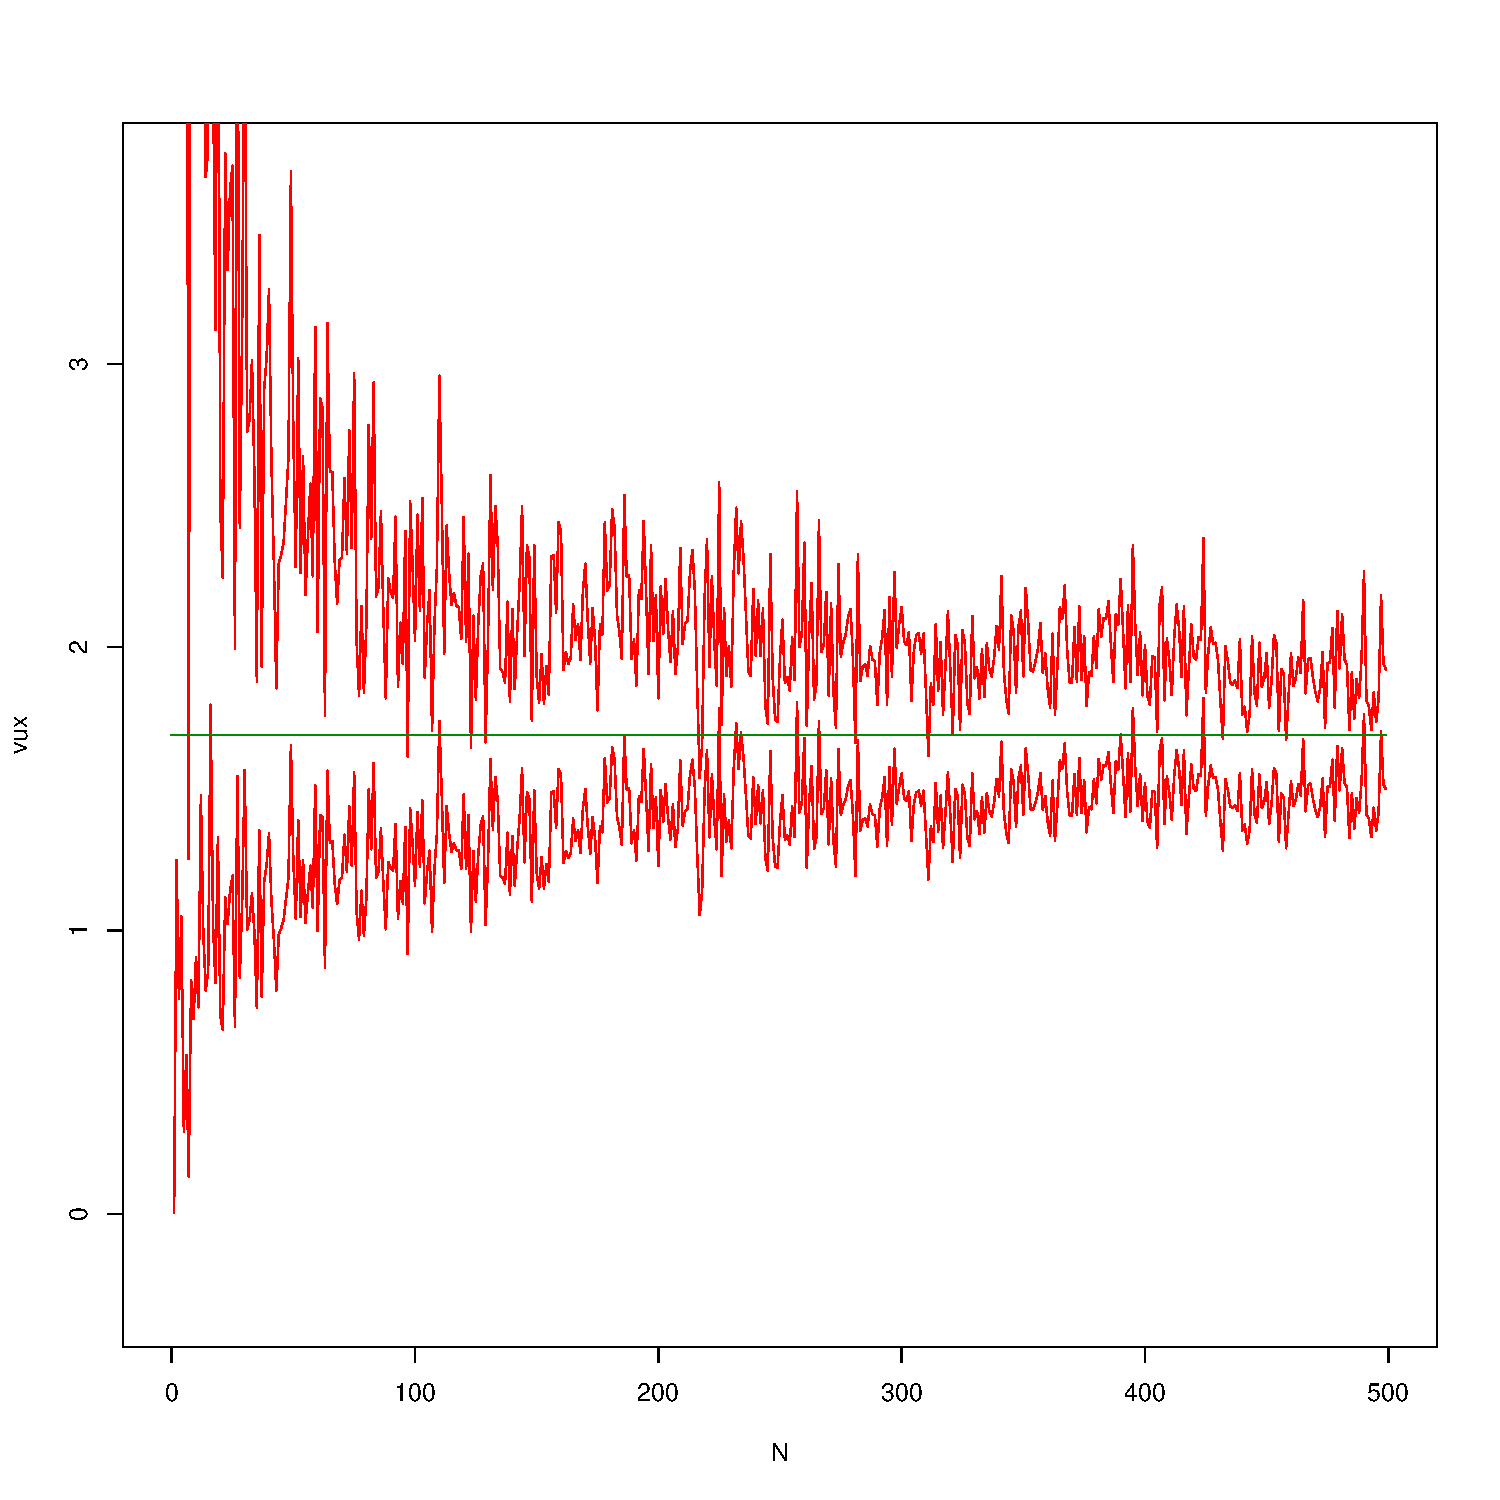
\includegraphics[width=.25\hsize]{img/vux-500.pdf}
	\caption{分散の区間推定 (95\%信頼区間)}
	\label{img:estimate-variance}
	\begin{minipage}{\hsize}
		\centering
		\begin{tabular}{c}
			\begin{minipage}{0.25\hsize}
				\centering
				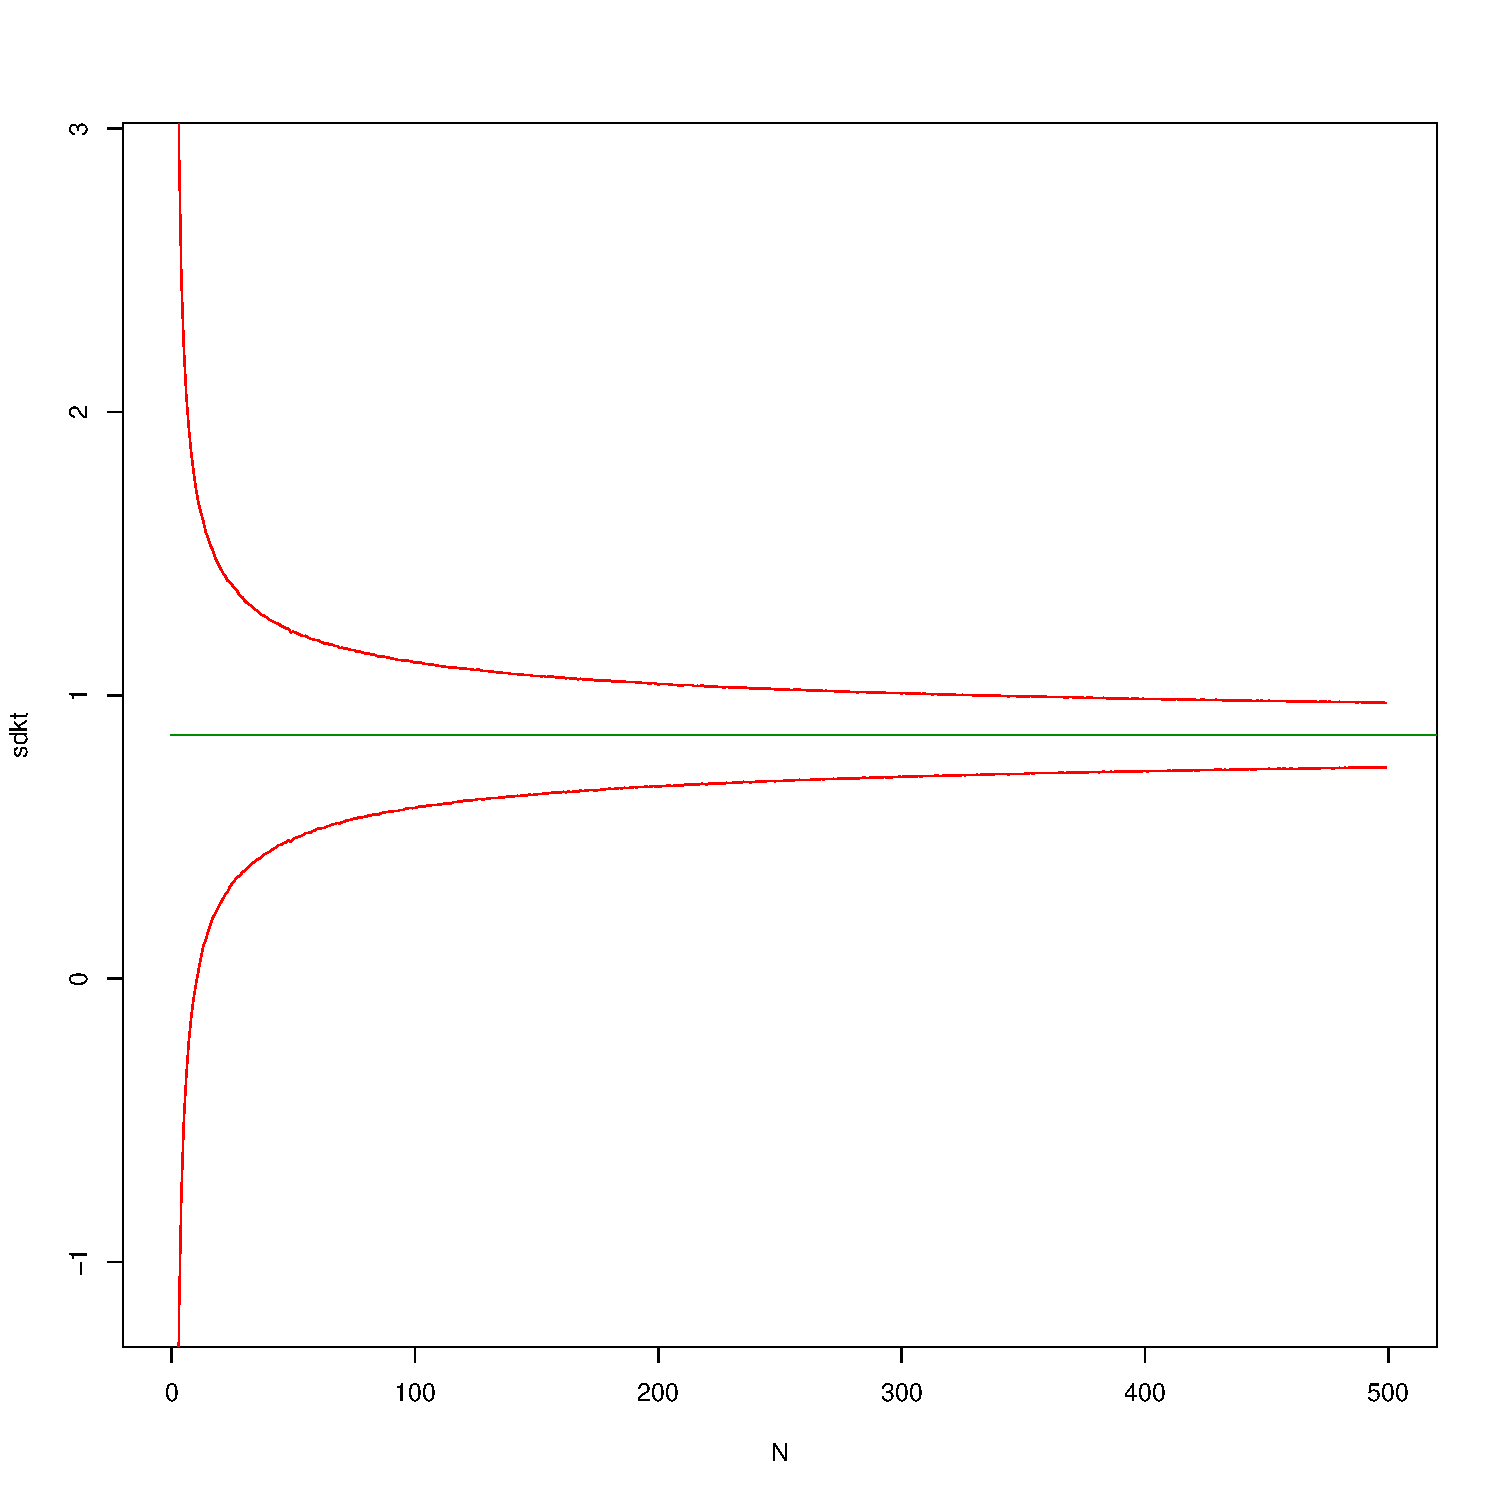
\includegraphics[width=\linewidth]{img/sdkt.pdf}
				\subcaption{既知の標準偏差使用\\(\emph{t}分布)}
				\label{img:sdkt-mean}
			\end{minipage}
			\begin{minipage}{0.25\hsize}
				\centering
				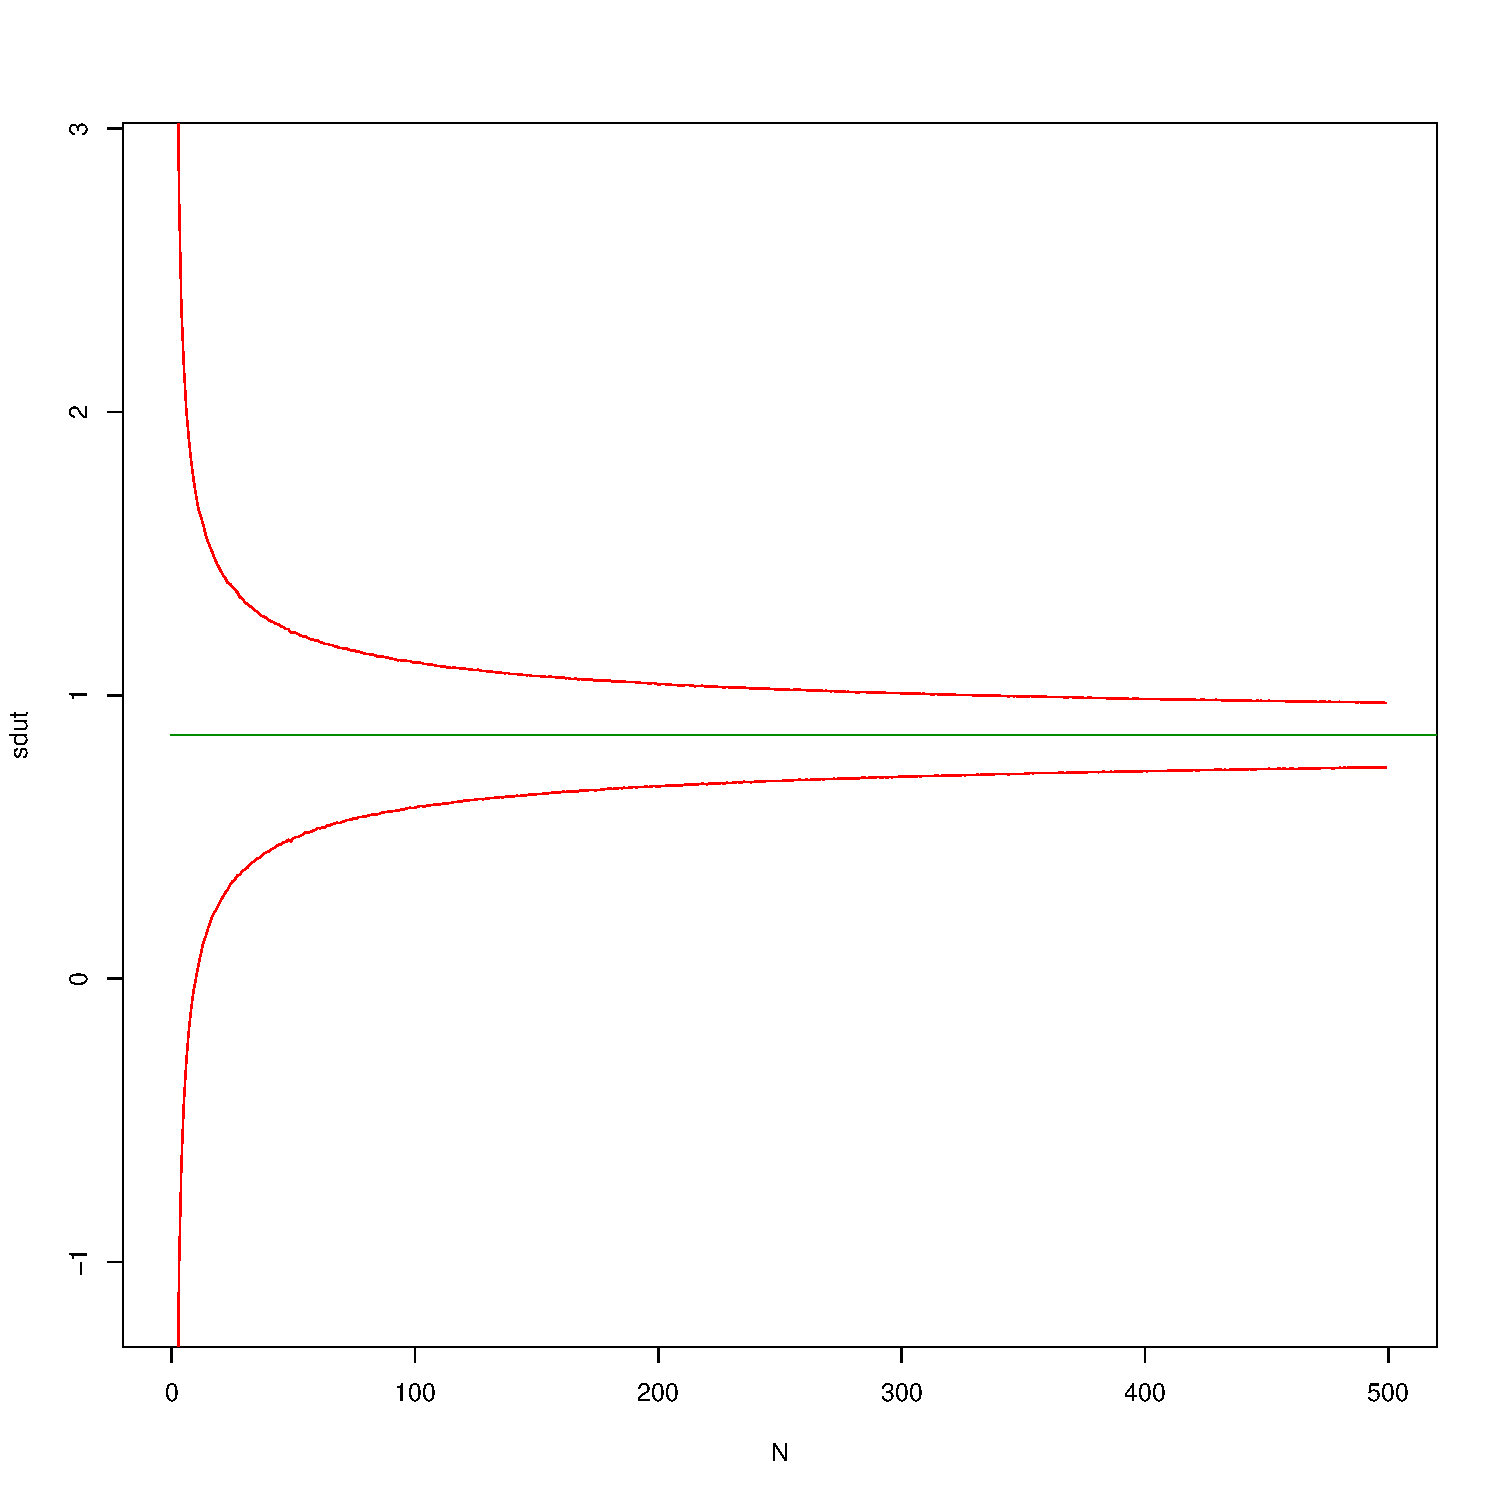
\includegraphics[width=\linewidth]{img/sdut.pdf}
				\subcaption{推定標準偏差使用\\(\emph{t}分布)}
				\label{img:sdut-mean}
			\end{minipage}
			\begin{minipage}{0.25\hsize}
				\centering
				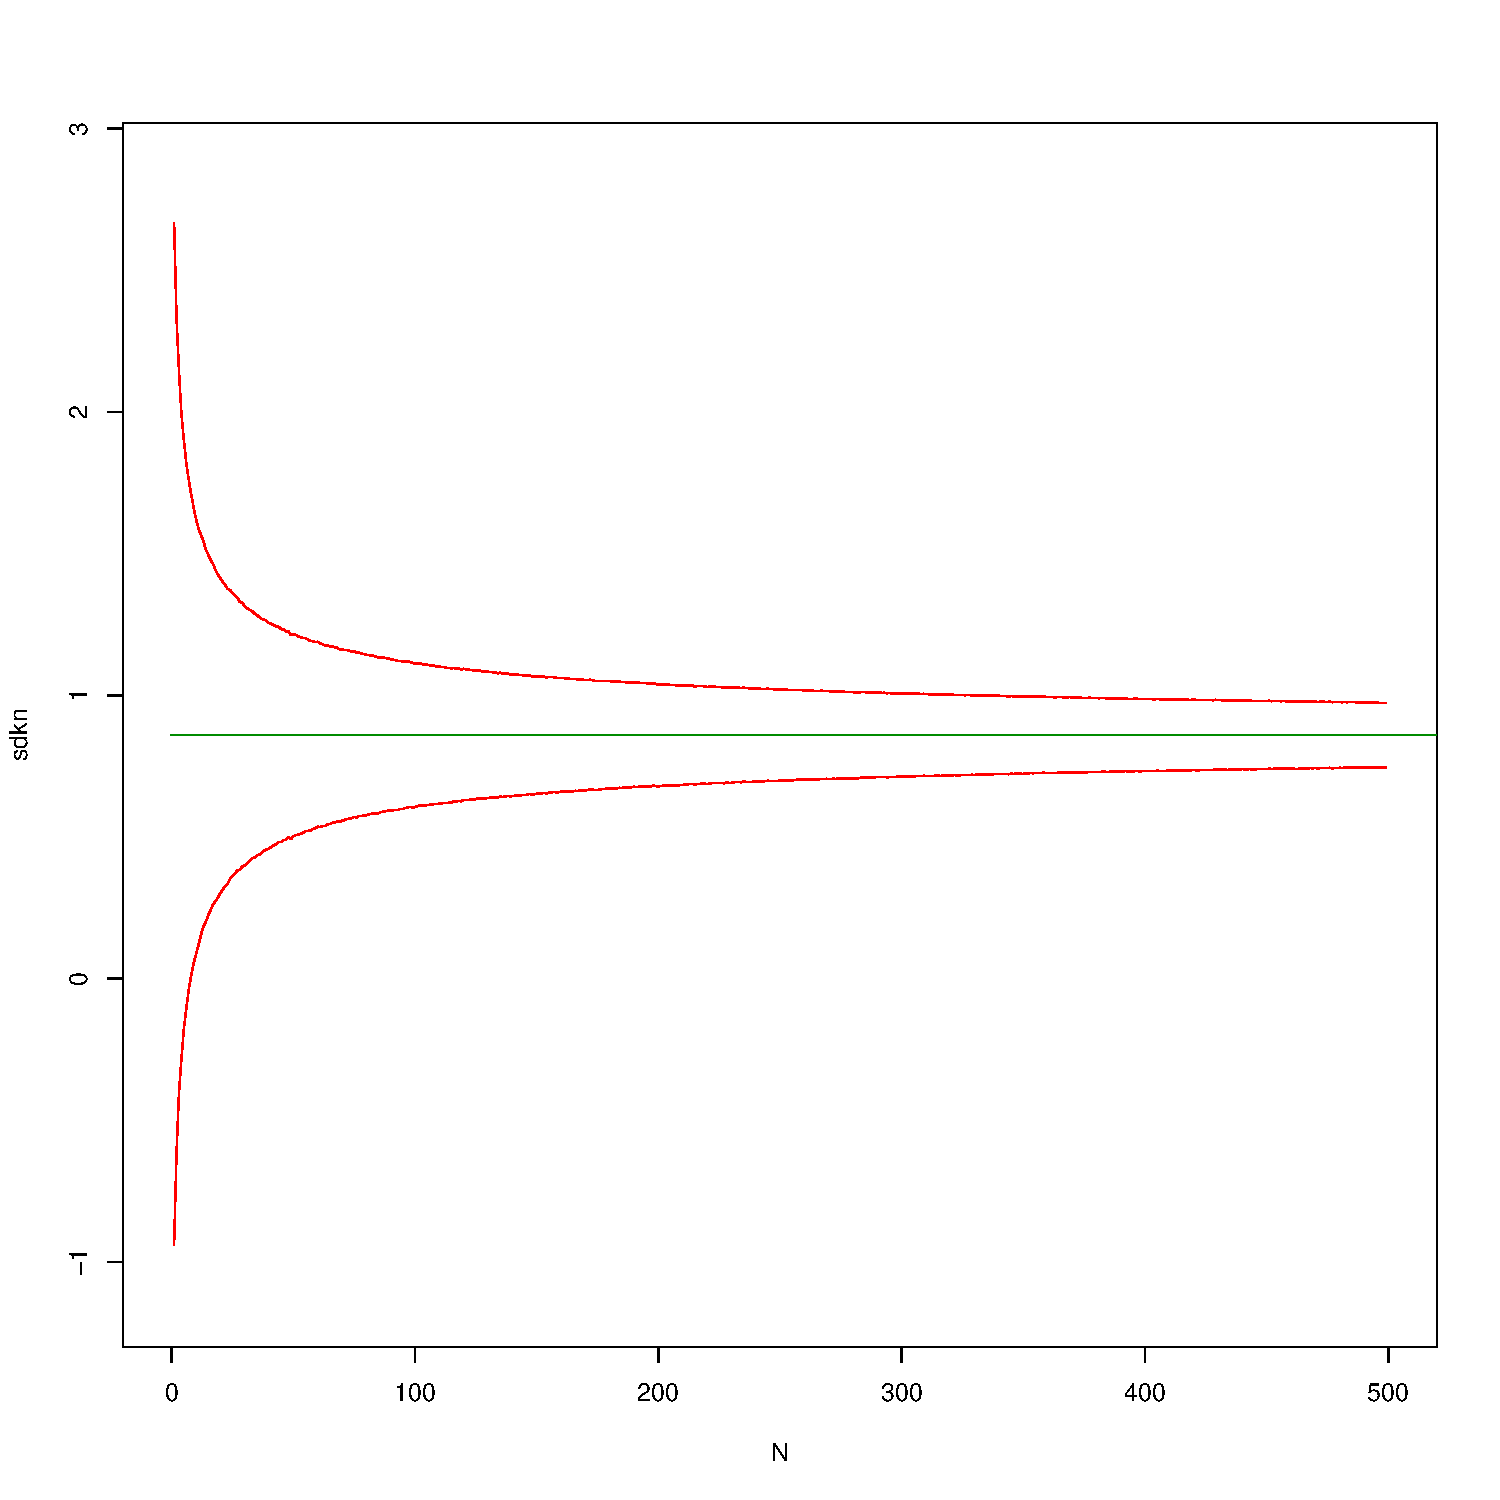
\includegraphics[width=\linewidth]{img/sdkn.pdf}
				\subcaption{既知の標準偏差使用\\(正規分布)}
				\label{img:sdkn-mean}
			\end{minipage}
			\begin{minipage}{0.25\hsize}
				\centering
				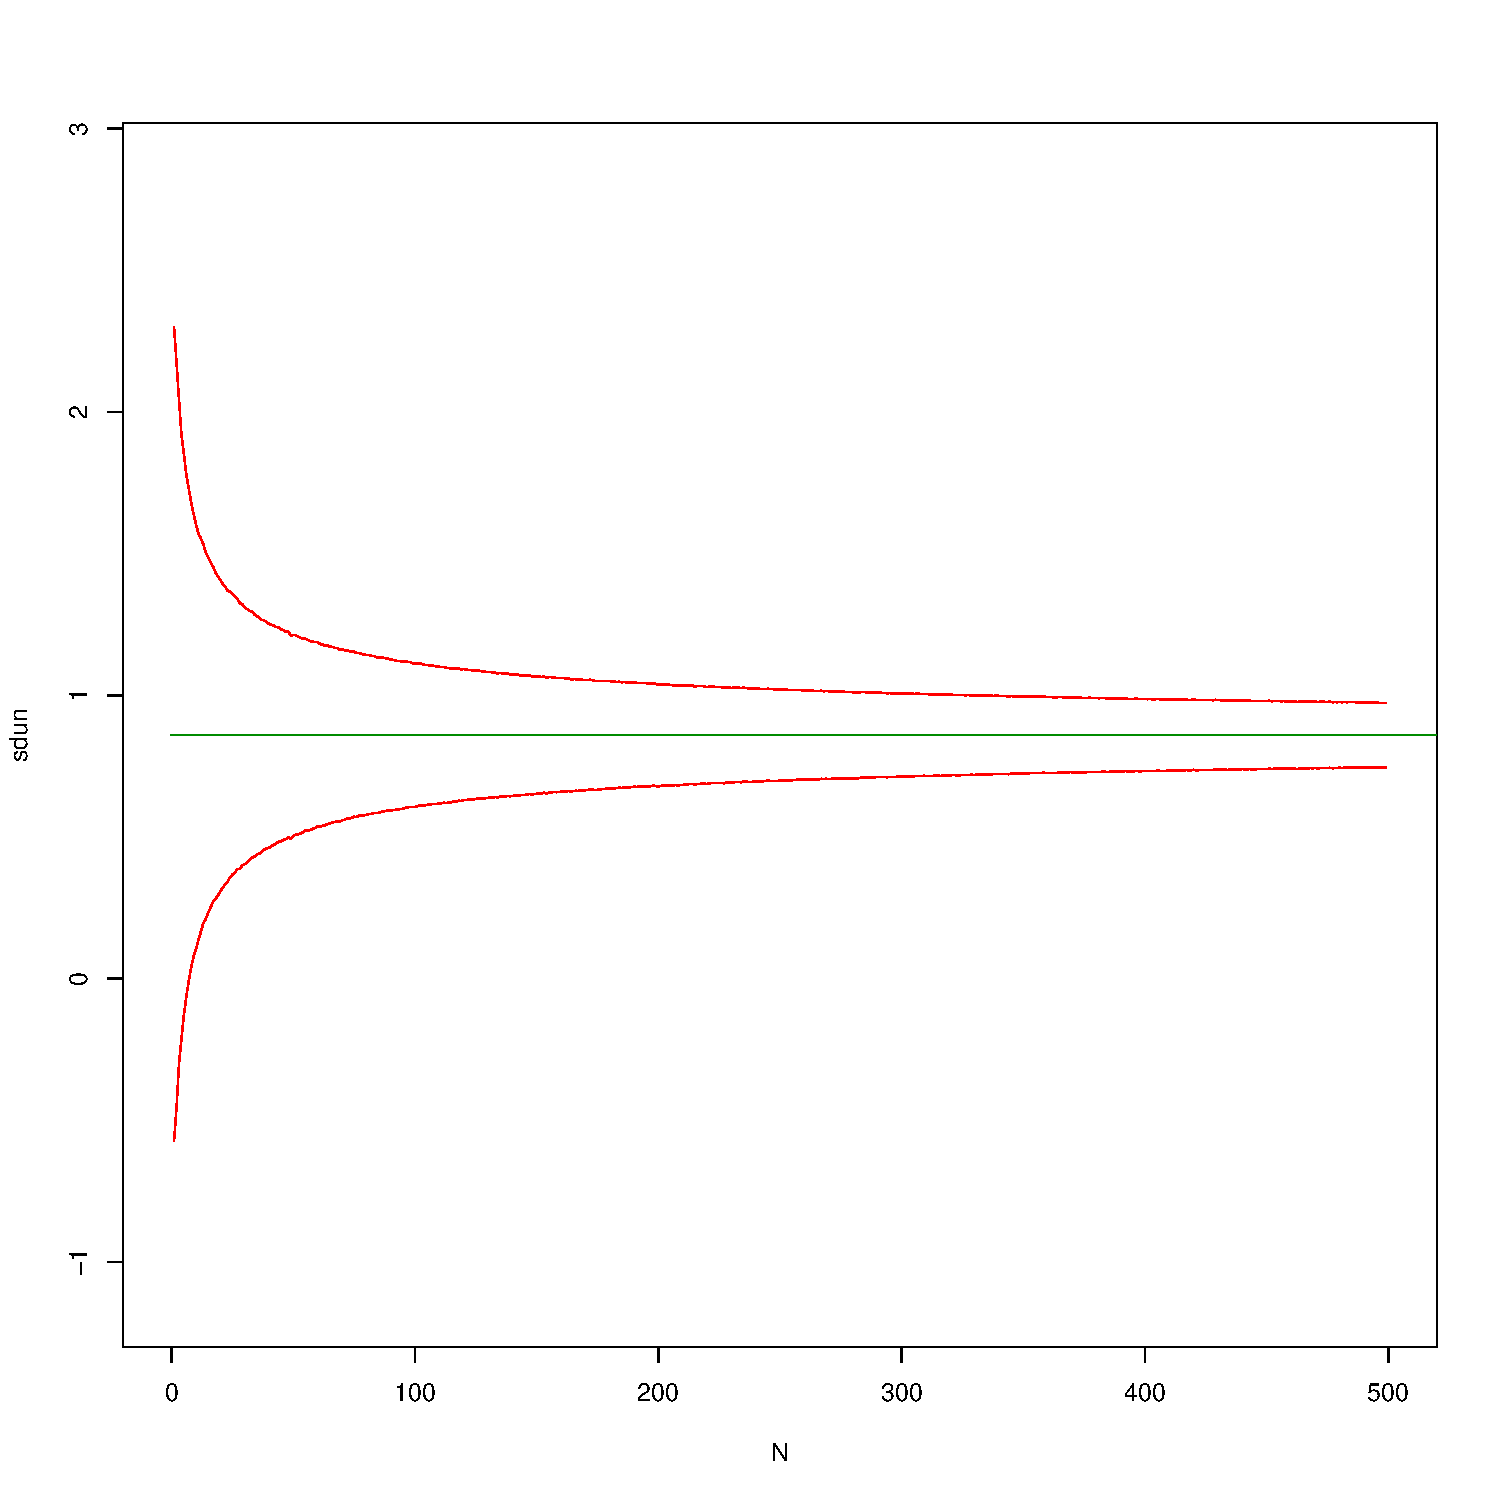
\includegraphics[width=\linewidth]{img/sdun.pdf}
				\subcaption{推定標準偏差使用\\(正規分布)}
				\label{img:sdun-mean}
			\end{minipage}
		\end{tabular}
		\caption{平均の区間推定の平均 (95\%信頼区間)}
		\label{img:estimate-mean-mean}
	\end{minipage}
	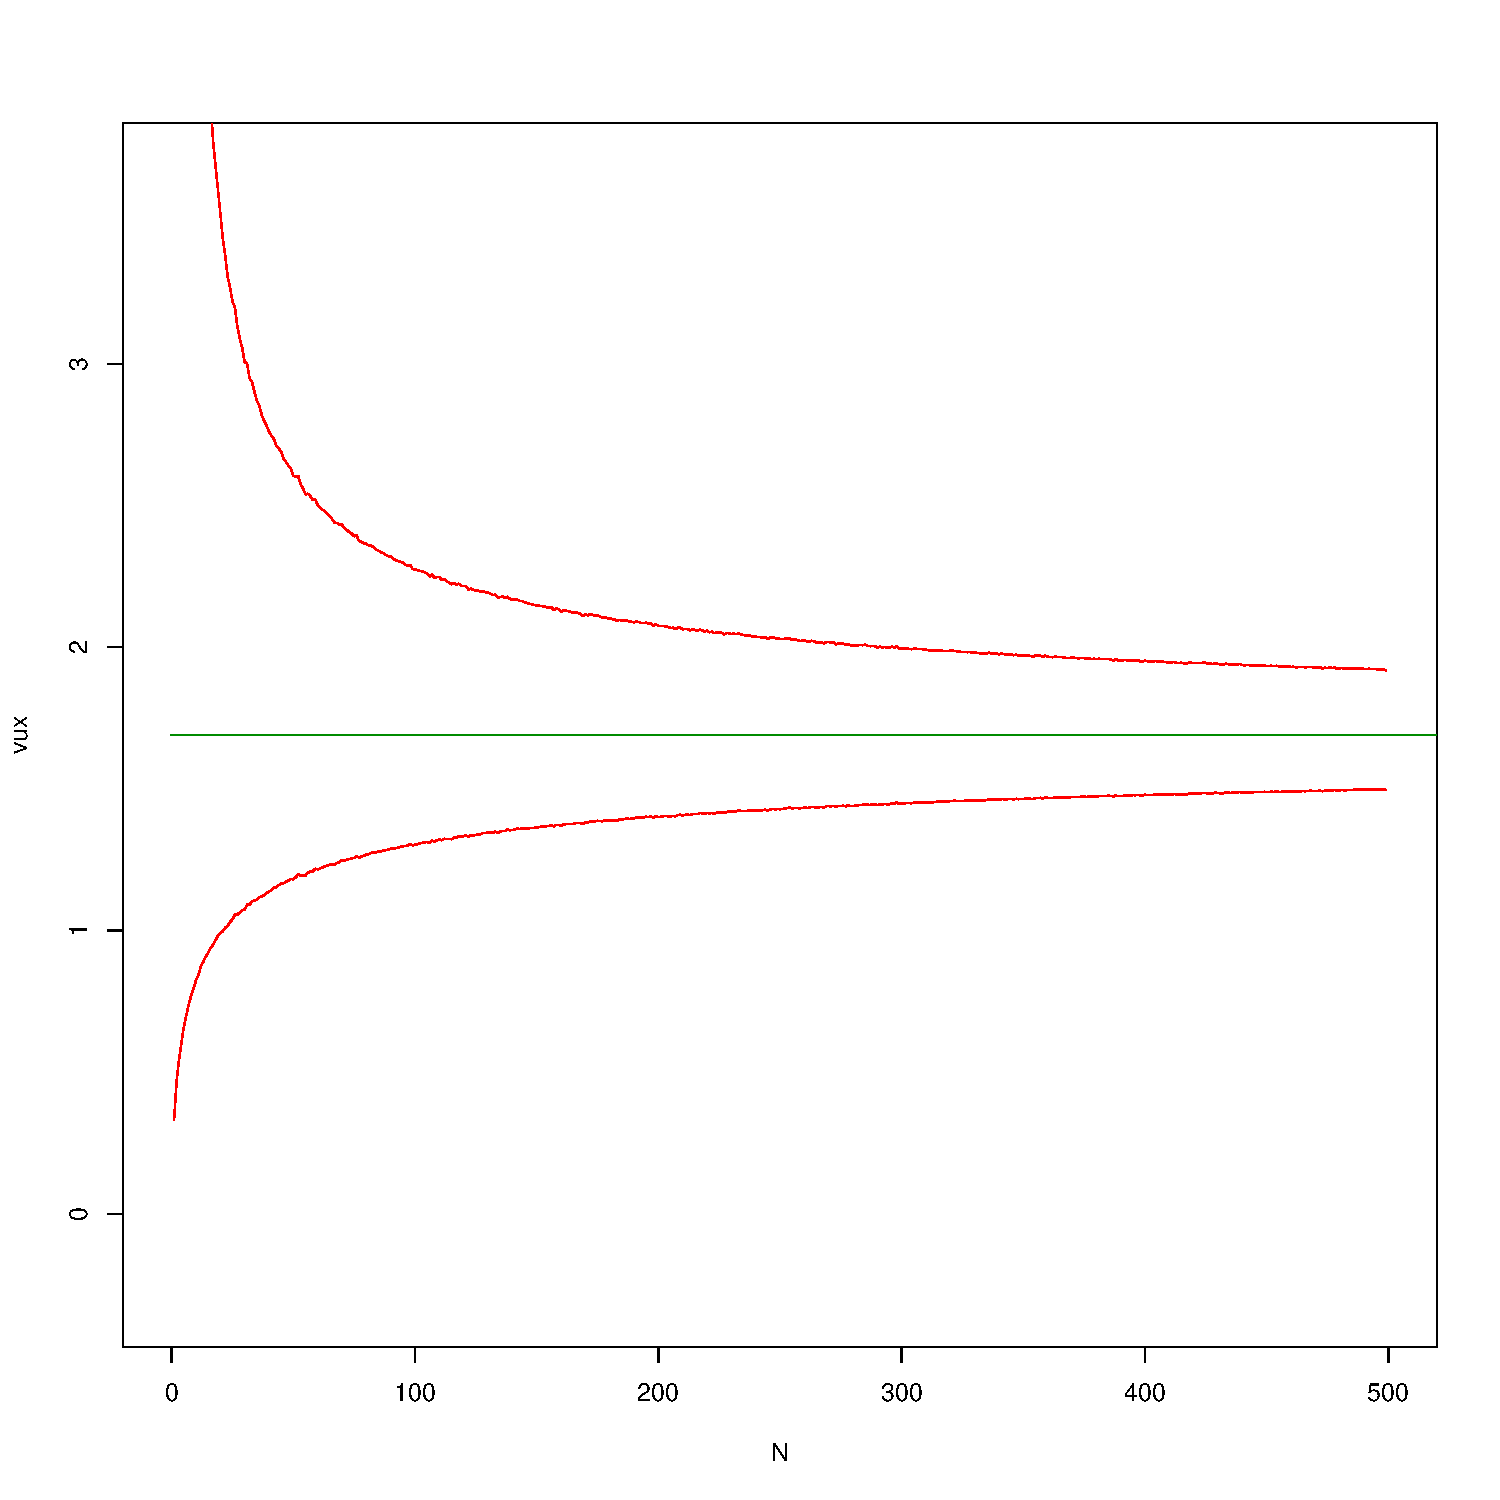
\includegraphics[width=.25\hsize]{img/vux.pdf}
	\caption{分散の区間推定の平均 (95\%信頼区間)}
	\label{img:estimate-variance-mean}
\end{figure}

\end{document}
